% šablona na pro bakalářskou práci na FAI UTB
% šablona je úpravou původní šablony pro FAI UTB
% =======================================================
% verze 0.9.5 (10. říjen 2005)
% autor: Ing. Jozef Říha ()
% některé komentáře převzaty z dokumentu Ivana Pomykacze
% =======================================================
% upravil Martin Zajíc
% šablona je upravena aby šla bez problému přeložit pomocí TeXlive a překladače XeLaTeX
% XeLaTex také řeší neduhy spojené s kódováním českých znaků a jejich kopírování z PDF dokumnetu
\documentclass[a4paper,12pt,twoside,BCOR=10mm]{article}
\usepackage{xltxtra}
\usepackage[czech]{babel}
\usepackage{listings}
\usepackage{indentfirst}
\usepackage{color}
\usepackage[svgnames]{xcolor} 
\usepackage{colortbl}
\usepackage{array}
\usepackage{graphicx}
\usepackage{amsmath}
\usepackage{fancyhdr}
\usepackage{fancyvrb}
\usepackage{fancybox,calc} 
\usepackage{hyperref}
\usepackage{multirow}
\usepackage{tocloft}
\usepackage{textcase}
\usepackage{ifthen}
\usepackage{setspace}
\usepackage{ccaption}
\usepackage{sectsty}
\usepackage{wrapfig}
%\usepackage[srcstyle=leftnumhang,linenumbersep={\ }]{examplep}
% ************************ NASTAVENÍ AUTORA A NÁZVU DOKUMENTU ************************
\newcommand{\rok}{2014}
\newcommand{\jmeno}{Martin Zajíc}
\newcommand{\typprace}{Diplomová práce}
\newcommand{\predmet}{Informační systém knihkupectví}
\newcommand{\predmeten}{přeložit}
% ************************ NASTAVENÍ TISKOVÉHO ZRCADLA ************************
\textheight=248mm
\textwidth=155mm
\voffset=-1.61cm
\oddsidemargin=0.96cm
\evensidemargin=0.96cm

% nastavení záhlaví
\headheight=0.5cm
\headsep=1cm

% nastavení zápatí
\footskip=1ex
\rhead{\thepage}
\cfoot{}
% "vypnout" poznámky na okrajích
\marginparpush=0mm
\marginparwidth=0mm
\marginparsep=0mm

\pagestyle{fancy}
% ****************** NASTAVENÍ HYPERPREF (BAREV ODKAZŮ, PDF DOKUMENTU) **************
\hypersetup{
    pdftoolbar=true,        % show Acrobat’s toolbar?
    pdfmenubar=true,        % show Acrobat’s menu?
    pdftitle={\typprace~-~\predmet },    % title
    pdfauthor={\jmeno},     % author
    pdfsubject={\predmet},   % subject of the document
    pdfcreator={\jmeno},   % creator of the document
    colorlinks=true,       % false: boxed links; true: colored links
    linkcolor=black,          % color of internal links
    citecolor=black,        % color of links to bibliography
    filecolor=black,      % color of file links
    urlcolor=black           % color of external links
}

% ****************** NASTAVENÍ PÍSMA, ODSTAVCE, ROVNIC, POZNÁMEK **************
\parindent=0em
\def\thefootnote{\arabic{footnote})}  % poznámka pod čarou se závorkou
\onehalfspacing % nastavím řádkování tímto způsobem nebo \renewcommand{\baselinestretch}{1.5} ??
\setlength{\parskip}{3pt}   % vertikální mezera mezi nadpisy
% *************************** NASTAVENÍ ČÍTAČŮ   ********************************
\setcounter{tocdepth}{3} % do obsahu se ukládají pouze první dvě úrovně kapitol

% *************************** UŽIVATELSKÉ STYLY *******************************
\newcommand{\nn}[1]{\clearpage\section*{\texorpdfstring{\uppercase{#1}}{#1}}\addcontentsline{toc}{section}{\uppercase{#1}}}% styl nn = nečíslovaný nadpis (je vysázený v obsahu)
\newcommand{\nm}[1]{\clearpage\section*{\uppercase{#1}}}  % definujeme styl nm = nečíslovaný nadpis (není vysázený v obsahu)
\newcommand{\nmm}[1]{\section*{#1}} % definujeme styl nmm = nečíslovaný nadpis (není vysázený v obsahu) malými písmeny bez clearpage
\newcommand{\nns}[1]{\section*{\uppercase{#1}}}   % definujeme styl ns = nečíslovaný nadpis na stejné stránce (není vysázený v obsahu)
\newcommand{\sectionV}[1]{\section{\uppercase{#1}}} %nadpis1 (section) velkým
%\renewcommand{\section}[1]{\section{\uppercase{#1}}}
\newcommand{\upc}[1]{\uppercase{#1}} %zjednodušení pro velká písmena
\newcommand{\odkazNaKapitolu}[1]{(viz.~kapitola~\ref{#1}/s\pageref{#1})}
\newcommand{\odkazNaObrazek}[1]{(viz.~obr.~\ref{#1}/s\pageref{#1})}

\newcommand{\nadpis}[1]{%nadpis pod kterym je vertikalni mezera
  \vspace{4 mm}
  \textbf{#1}\\
  \vspace{4 mm}
  }

\newcommand{\obr}[3]{% styl \obr pro obrázky
  \begin{figure}[h]
  \center\includegraphics[scale=#2]{#1}
  \caption{#3}
  \end{figure}
  }

\newcommand{\ofZadani}[2]{% styl \obr pro obrázky
  \begin{figure}[h]
  \center\includegraphics[width=500pt,height=700pt]{#1}
  %\caption{#2}
  \end{figure}
  }

\newcommand{\tab}[3]{% styl \tab pro tabulky
  \begin{table}[h]
  \caption{#1}
  \begin{center}
  \begin{tabular}{#2}
  #3
  \end{tabular}
  \end{center}
  \end{table}
  }

\newcommand{\tabpri}[3]{% styl \tabpri pro tabulky v příloze
  \begin{table}[h]
  \begin{center}
  #1
  \end{center}
  \begin{center}
  \begin{tabular}{#2}
  #3
  \end{tabular}
  \end{center}
  \end{table}
  }

\newcommand{\rov}[2][chybějici rovnice]{% styl \rov pro rovnice
  \begin{equation}
  #2
  \label{#1}
  \end{equation}
  }
  
\newcommand{\seznamobr}{% příkaz \seznamobr pro vysázení seznamu obrázků
  \addcontentsline{toc}{section}{\listfigurename}
  \clearpage
  \listoffigures
  \clearpage
  }

\newcommand{\seznamtab}{% příkaz \seznamtab pro vysázení seznamu obrázků
  \addcontentsline{toc}{section}{\listtablename}
  \clearpage
  \listoftables
  \clearpage
  }
  
\newcommand{\seznamlit}[1]{% příkaz \seznamlit pro vysázení seznamu literatury
  \addcontentsline{toc}{section}{\refname}
  \begin{thebibliography}{10}
  #1
  \end{thebibliography}}
  
\newcommand{\seznamzkr}{% příkaz \seznamzkr pro přípravu seznamu použitých zkratek a symbolů
  \nn{Seznam použitých symbolů a zkratek}
  }
  
\newcommand{\obsah}{% \obsah vysází obsah v daném místě
  \clearpage
  \thispagestyle{empty}
  \tableofcontents
  \clearpage
  \pagestyle{fancy}
  }

\renewcommand{\b}[1]{\textbf{#1}} % \b = tučně
\newcommand{\bi}[1]{\textbf{\textit{#1}}} % \bi = tučná kurzíva
\renewcommand{\it}[1]{\textit{#1}}    % \it = kurzíva
  
% ******* NASTAVENÍ ZOBRAZENÍ PŘÍLOH -- SEZNAM, ČÍSLOVÁNÍ, VLASTNÍ STYL *******
\makeatletter % tímto příkazem dávám najevo, že budu editovat přímo příkazy ze šablony

% definice seznamu příloh - příkaz \listofappendices
\newcommand{\listofappendices}{%
  \newpage
  \setcounter{section}{0}
  \nn{Seznam příloh}
  \@restonecolfalse\if@twocolumn\@restonecoltrue\onecolumn\fi
  \@mkboth{LIST OF APPENDICES}{LIST OF APPENDICES}
  \@starttoc{loa}\if@restonecol\twocolumn\fi
  \pagestyle{empty}
  \thispagestyle{fancy}
  }

\def\ext@appendix{loa}
\def\tocname{loa}

% definice příkazu \priloha{nazev prilohy} pro vložení nové přílohy
\newcommand{\priloha}[1]{
  \clearpage
  \refstepcounter{section}
  \addtocontents{loa}{\protect\makebox[1.5cm][l]{P \@Roman\c@section.} #1\newline}
{\bf PŘÍLOHA P \@Roman\c@section. \uppercase{#1}}\par\vspace{0.5cm}}

% v obsahu nastavím VELKÉ PÍSMENA pro styl část
\renewcommand{\part}[1]{
  \refstepcounter{part}
  \addcontentsline{toc}{section}{\thepart~~\uppercase{#1}}%
\clearpage
\normalfont
  \vspace*{9cm}
  \begin{center}\huge \bfseries\thepart. \uppercase{#1}\end{center}%
  \markboth{}{}\par
\nobreak
\clearpage  
}
% *******************Barevný code *******************
\definecolor{codeback}{gray}{0.8} %barva pozadi

\newenvironment{codeframe}{% 
  \begin{Sbox} 
    \begin{minipage} 
      {\columnwidth-\leftmargin-\rightmargin-2\fboxsep-2\fboxrule-4pt} 
}{% 

  \end{minipage} 
  \end{Sbox} 
  \begin{center} 
    \fcolorbox{black}{codeback}{\TheSbox} 
  \end{center} 
} 

% *************** NASTAVENÍ FORMÁTU ČÍSLOVÁNÍ OBRÁZKŮ A TABULEK ***************
\def\thefigure{\arabic{figure}}      % číslování obrázků typu (y)
\def\thetable{\arabic{table}}        % číslování tabulek typu (y)
\captiondelim{. } % změníme dvoutečku za Obr/Tab za tečku

% ***************************** VYNULOVÁNÍ ČÍTAČŮ *****************************
\@addtoreset{table}{section}    % vynulování čítače
%\@addtoreset{figure}{section}   % vynulování čítače
\@addtoreset{footnote}{section} % vynulování čítače
  
\makeatother % a to je ukončení \makeatletter

% ************* ÚPRAVA VZHLEDU OBSAHU, SEZNAMU OBRÁZKÙ A TABULEK **************
% nastavení vertikální mezery před stylem část, nadpis 1--3
\setlength{\cftbeforepartskip}{3pt}
\setlength{\cftbeforesecskip}{3pt}
\setlength{\cftbeforesubsecskip}{3pt}
\setlength{\cftbeforesubsubsecskip}{0cm}
% odsazení zleva pro styl část, nadpis 1--3
\setlength{\cftpartindent}{0cm}
\setlength{\cftsecindent}{0cm}
\setlength{\cftsubsecindent}{0cm}
\setlength{\cftsubsubsecindent}{0cm}
% nastavení fontu pro styl část, nadpis 1--3
\renewcommand{\cftpartfont}{\small\bfseries}
\renewcommand{\cftsecfont}{\small\bfseries}
\renewcommand{\cftsubsecfont}{\scshape}
\renewcommand{\cftsubsubsecfont}{}
% odsazení čísla a textu titulku pro styl část, nadpis 1--3
\cftsetindents{part}{0cm}{1cm}
\cftsetindents{sec}{0cm}{1cm}
\cftsetindents{subsec}{1cm}{1.5cm}
\cftsetindents{subsubsec}{1.2cm}{1.7cm}
\cftsetindents{fig}{0cm}{1.5cm}
\cftsetindents{tab}{0cm}{1.5cm}
% nastavení vodící čáry pro styl část, nadpis 1--3, obrázky a tabulky
\renewcommand{\cftdot}{\ensuremath{.}} % tímto příkazem lze změnit vodící tečky v obsahu na jiný znak
\renewcommand{\cftpartleader}{\cftdotfill{0.3}}
\renewcommand{\cftsecleader}{\cftdotfill{0.3}}
\renewcommand{\cftsubsecleader}{\cftdotfill{0.3}}
\renewcommand{\cftsubsubsecleader}{\cftdotfill{0.3}}
\renewcommand{\cftfigleader}{\cftdotfill{0.3}}
\renewcommand{\cfttableader}{\cftdotfill{0.3}}
% změna fontu pro text "Obsah", "Seznam obrázků" a "Seznam tabulek"
\renewcommand{\cfttoctitlefont}{\normalsize\bfseries\thispagestyle{empty}}
\renewcommand{\cftloftitlefont}{\normalsize\bfseries\thispagestyle{fancy}}
\renewcommand{\cftlottitlefont}{\normalsize\bfseries\thispagestyle{fancy}}
\renewcommand{\cftfigpresnum}{Obr. }
\renewcommand{\cftfigaftersnum}{.}
\renewcommand{\cfttabpresnum}{Tab. }
\renewcommand{\cfttabaftersnum}{.}

% ************************ NASTAVENÍ FONTU PRO NADPISY ************************
\sectionfont{\normalsize}
\subsectionfont{\normalsize\bfseries} 
\subsubsectionfont{\normalsize\bfseries}
\paragraphfont{\small\bf}
% definice nového stylu \comment -- komentář k šabloně
%\newcommand{\comment}[1]{\color{red}#1\color{black}}

% ****************************** KONEC PREAMBULE ******************************
\begin{document}
% ****************************** Vlastní definice ******************************
% ********* musí být na začátku dokumnetu v preambuli nefungují ****************
\renewcommand{\refname}{\texorpdfstring{\uppercase{Seznam použité literatury}}{Seznam použité literatury}}
\renewcommand*{\listfigurename}{\texorpdfstring{\uppercase{Seznam obrázků}}{Seznam obrázků}}
\renewcommand{\contentsname}{\texorpdfstring{\uppercase{Obsah}}{Obsah}}
\renewcommand*{\listtablename}{\texorpdfstring{\uppercase{Seznam tabulek}}{Seznam tabulek}}
\renewcommand*{\tablename}{Tab.}
\renewcommand\figurename{Obr.}
%********************************* Hlavička ************************************
\lhead{\b{UTB ve Zlíně, Fakulta aplikované informatiky}}

\thispagestyle{empty}
\voffset=-2.01cm\evensidemargin=0pt\oddsidemargin=0cm\parindent=0pt\headsep=0pt\headheight=0pt\parskip=0pt\textheight=272mm\textwidth=200mm
\renewcommand{\baselinestretch}{0}
%********************************* Úvodní stránka s logem fakulty ********************
\setlength{\unitlength}{1mm}
\begin{picture}(-10,8)
\put(0,-50){\makebox(170,50){}}
%*******************************Uvodni stranka z nazvem prace na dva radky*********
%\put(0,-100){\makebox(170,50){\fontsize{24}{1}\b{\textsf{Zálohovací server založený na}}}}
%\put(0,-110){\makebox(170,50){\fontsize{24}{1}\b{\textsf{GNU/Linux Debian}}}}
%\put(0,-130){\makebox(170,50){\fontsize{20}{1}\b{\textsf{Backup server based on GNU/Linux Debian}}}}
%\put(0,-150){\makebox(170,25){\fontsize{20}{1}\b{\textsf{\jmeno}}}}
%*******************************konec uvodni stranka na dva radky***********************
\put(0,-115){\makebox(170,50){\fontsize{24}{1}\b{\textsf{\predmet}}}}
% \put(0,-130){\makebox(170,50){\fontsize{22}{1}\b{\textsf{\predmeten}}}}
\put(0,-150){\makebox(170,25){\fontsize{20}{1}\b{\textsf{\jmeno}}}}
\put(82.2,-223.3){\makebox(84,16.4){
\includegraphics[width=84mm]{fai_logo_cz.png}}}
\put(0,-205){\linethickness{1pt}\line(1,0){170}}
\put(4,-215){\makebox(69.5,4.5)[l]{\noindent\fontsize{16}{1}\b{\textsf{\typprace}}}}
\put(4,-220){\makebox(69.5,4.5)[l]{\noindent\fontsize{16}{1}\b{\textsf{\rok}}}}
\put(0,-225){\linethickness{1pt}\line(1,0){170}}
\put(75,-223.3){\linethickness{1pt}\line(0,1){16.4}}
\end{picture}
%********************************* nascanované zadání ************************************
\clearpage
\thispagestyle{empty}
\ofZadani{./img/ofZadani/ofZadaniStr1.png}{Oficiální zadání bakalářské práce strana 1}
\clearpage
\thispagestyle{empty}
\ofZadani{./img/ofZadani/ofZadaniStr2.png}{Oficiální zadání bakalářské práce strana 2}
%********************************* Abstrakt ************************************
\clearpage
\thispagestyle{empty}
\voffset=-1.61cm\evensidemargin=0.96cm\oddsidemargin=0.96cm\headsep=1cm\headheight=0.5cm\setlength{\parskip}{3pt}\textheight=248mm\textwidth=155mm
\nm{\uppercase{Abstrakt - smazat}}
\vspace{1cm}
text
\vspace{1cm}

\emph{Klíčová slova:} Linux, distribuce, BASH, LFS, LiveCD, bezpečnost Linuxu, kompilace, DAC, MAC
\vspace{2cm}

%********************************* poděkování, motto, úryvky knih, básní atp. ************************************
\clearpage
\thispagestyle{empty}
 - smazat

\vspace{3cm}
"Nejlepší knihy jsou takové, které člověku říkají, co už sám ví."\\

\hspace{9cm}GEORGE ORWELL
%********************************* Prohlášení ************************************
\clearpage
\thispagestyle{empty}
\clearpage
\nmm{Prohlašuji, že}
\begin{itemize}\fontsize{10}{1}
\normalsize
\item beru na vědomí, že odevzdáním bakalářské práce souhlasím se zveřejněním své práce podle zákona č. 111/1998 Sb. o vysokých školách a o změně a doplnění dalších zákonů (zákon o vysokých školách), ve znění pozdějších právních předpisů, bez ohledu na výsledek obhajoby;
\item beru na vědomí, že bakalářská práce bude uložena v elektronické podobě v univerzitním informačním systému dostupná k prezenčnímu nahlédnutí, že jeden výtisk bakalářské práce bude uložen v příruční knihovně Fakulty aplikované informatiky Univerzity Tomáše Bati ve Zlíně a jeden výtisk bude uložen u vedoucího práce; 
\item byl/a jsem seznámen/a s tím, že na moji bakalářskou práci se plně vztahuje zákon č. 121/2000 Sb. o právu autorském, o právech souvisejících s právem autorským a o změně některých zákonů (autorský zákon) ve znění pozdějších právních předpisů, zejm. § 35 odst. 3;
\item beru na vědomí, že podle § 60 odst. 1 autorského zákona má UTB ve Zlíně právo na uzavření licenční smlouvy o užití školního díla v rozsahu § 12 odst. 4 autorského zákona;
\item beru na vědomí, že podle § 60 odst. 2 a 3 autorského zákona mohu užít své dílo –bakalářskou práci nebo poskytnout licenci k jejímu využití jen s předchozím písemným souhlasem Univerzity Tomáše Bati ve Zlíně, která je oprávněna v takovém případě ode mne požadovat přiměřený příspěvek na úhradu nákladů, které byly Univerzitou Tomáše Bati ve Zlíně na vytvoření díla vynaloženy (až do jejich skutečné výše);
\item beru na vědomí, že pokud bylo k~vypracování bakalářské práce využito softwaru poskytnutého Univerzitou Tomáše Bati ve Zlíně nebo jinými subjekty pouze ke studijním a~výzkumným účelům (tedy pouze k~nekomerčnímu využití), nelze výsledky bakalářské práce využít ke komerčním účelům;
\item beru na vědomí, že pokud je výstupem bakalářské práce jakýkoliv softwarový produkt, považují se za součást práce rovněž i~zdrojové kódy, popř. soubory, ze kterých se projekt skládá. Neodevzdání této součásti může být důvodem k~neobhájení práce.
\end{itemize}
\nmm{Prohlašuji,}
\begin{itemize}
 \normalsize
\item že jsem na bakalářské práci pracoval samostatně a použitou literaturu jsem citoval. V případě publikace výsledků budu uveden jako spoluautor.
\item že odevzdaná verze bakalářské práce a verze elektronická nahraná do IS/STAG jsou totožné.
\end{itemize}
\vspace{1cm}
\begin{tabular}{lc}
Ve Zlíně &\hspace{9cm} .......................\\
~ &\hspace{9cm} podpis diplomanta
\end{tabular}

% obrázky \obr{soubor.png}{scale}{popisek}
% tabulky \tab{popisek}{nastaveni}{obsah}
% tabulky v příloze \tabpri{vrch tabulky}{nastaveni}{obsah}
% rovnice \rov{popisek}{obsah}
% tučně \b{tučné}
% tučná kurzíva \bi{tučná kurzíva}
% kurzíva \it{kurzíva}
% citace text~\cite{zkratka knihy}
%********************************* Generování obsahu ************************************
\obsah
%********************************* úvod ************************************
\nn{Úvod}
 - smazat

%********************************* Vlastní obsah ************************************
%********************************* Teoretická část ************************************
\part{Teoretická část}

\section{\upc{Knihovní informační systém}}
Informační systémy obecně se stávají velmi komplexním řešením pro kompletní vedení firem jakýchkoliv rozměrů, zajišťují širokou škálu služeb, od komunikace se zákazníky přes ekonomické systémy až po prodej a~tvorbu obsahu nebo pro evidenci skadu. Takové systémy jsou vyvíjeny většinou dlouhodobě na míru zákazníkovi a~rozvíjeny společně s~jeho růstem a~potřebám. Nebo sa také jedná o~různá spojení stávajících informačních systémů, která jsou často spravována separátně a~nenabízí přehled a~porovnání údajů jednotlivých částí.\\

\subsection{Existující informační systémy pro knihovny a kohkupectví}
Velmi častou aplikací, která se používá v~české republice je kombinace účetního systému Pohoda \href{http://www.ucetni-systemy.cz/pohoda-standard/c-4468/}{http://www.ucetni-systemy.cz/pohoda-standard/c-4468/}, která obsahuje kompletní správu pro firmu včetně pokladen skladů a~účetnictví a~dokáže tato data synchronizovat s~některým s~e-shopů např. PrestaShop \href{http://www.prestashop.com/}{http://www.prestashop.com/}. E-comerce a~komunikace se zákazníkem je pak na e-shopu, který většinou slouží pro klasický prodej. Komunikace mezi zaměstnanci probíhá prostřednictvím e-mailů nebo IM a~komunikace se zákazníkem, buď pomocí e-mailů nebo "chatu" přímo v~okně prohlížeče.\\

Další systémy jsou na tom podobně, co ovšem chybí je např. komunikace s~tvůrcem a~přehledu pro něj, jak se prodává jeho dílo. Nebo přímo rozhraní pro tvorbu knihy online.\\

\subsection{Trendy v informačních systémech}
Svět informačníčh systému se stále rychle vyvíjí, dříve byl vyspělý informační systém \it{DOSový} program, který se připojil na server, mnohdy ani to ne, a~obsluha jej ovládala klávesnicí. Dnes jsou požadavky na informační systémy mnohem větší a~zákazníci ve většině případů vyžadují dostupnost kdekoliv na světě pomocí webového prohlížeče v~mobilu nebo~tabletu.\cite{trendsIS}\\

Dalším trendem jsou sociální sítě jako Facebook,LinkedIn,Twitter apd,… informační systémy v~dnešní době zahrnují podpodu pro sociální síťe. Ale nejedná se pouze o~dnes velmi populární přihlašování bez nutnosti \it{"registrace"}, ale~např. zkoumání povědomí o~značce nebo komunikaci se zákazníky pomocí sociálních sítí a~realtime chatu.\cite{trendsIS}\\

\subsection{Proces schvalování knih}\label{sec:schvalovani}


\section{\upc{Použité technologie}}
K~vývoji bylo využito aktuálních nástrojů používaných pro vývoj moderních webových aplikací, které usnadňují práci programátorům a~zrychlují razantně tvorbu aplikace. Důraz je kladen na rychlost a~škálovatelnost takové aplikace.\\

\section{\upc{COFFEE-SCRIPT}}
\begin{figure}[h]
\begin{center}$
\begin{array}{c}

\includegraphics[scale=0.5]{./img/coffeescript.jpg}
\end{array}$
\end{center}
\caption[Logo coffeescript]{Logo coffeescript}
\end{figure}
Coffee-script je malý a~jednoduchý jazyk, který je traspiluje \footnote{transpilovat znamená převádět kód z jednoho programovačího jazyka na druhý} do javascriptu. Přispívá k~jednoduchosti kódu a~urychluje jeho psaní, protože vypouští závorky, přidává některou fukcionalitu ES6 \footnote{ES6 neboli ECMAScript6 je nástupce současného standardu ECMAScript5 používaného většnou prohlížečů, přináší podporu pro třídy,moduly, iterátor, yield, a další.} výrazně zjednodušuje cykly a~mnoho dalšího,…\\

\subsection{Několik ukázek kódu v coffeescriptu/javascriptu}
Přiřazení
     \begin{codeframe} 
      \begin{Verbatim}{frame=single}
#coffeescript
number   = 42
opposite = true

#javascript
var number = 42;
var opposite = true;
\end{Verbatim} 
    \end{codeframe}

Podmínky
     \begin{codeframe} 
      \begin{Verbatim}{frame=single}
#coffeescript
number = -42 if opposite
#number je -42 pokud je oppsite true
date = if friday then sue else jill
#pokej je friday tak date je sue jinak jill

#javascript - stejný kód
if (opposite) {
  number = -42;
}
date = friday ? sue : jill;
\end{Verbatim} 
    \end{codeframe}

Funkce není třeba psát složenými závorkami vše s indentací patří do funkce.
     \begin{codeframe} 
      \begin{Verbatim}{frame=single}
#coffeescript
square = (x) ->
  x * x

#javascript
var square = function(x) {
  return x * x;
};
\end{Verbatim} 
    \end{codeframe}

Objekty - objekty není třeba uzávírat do složených závorek.
     \begin{codeframe} 
      \begin{Verbatim}{frame=single}
#coffeescript
math =
  root:   Math.sqrt
  square: square
  cube:   (x) -> x * square x

#javascript
var math = {
  root: Math.sqrt,
  square: square,
  cube: function(x) {
    return x * square(x);
  }
};
\end{Verbatim} 
    \end{codeframe}

Testování existence proměnné - otazník za promněnnou testuje její existanci a~pokud elvis existuje vyskocí alert.
     \begin{codeframe} 
      \begin{Verbatim}{frame=single}
#coffeescript
alert "I knew it!" if elvis?

#javascript
if (typeof elvis !== "undefined" && elvis !== null) {
  alert("I knew it!");
}
\end{Verbatim} 
    \end{codeframe}

Cykly
     \begin{codeframe} 
      \begin{Verbatim}{frame=single}
#coffeescript
eat =(food)->
  console.log(food)

foods = ['broccoli', 'spinach', 'chocolate']
eat food for food in foods when food isnt 'chocolate'
#eat(food) je zavolána pokud položka v poli není chocolate
#Výstup:
broccoli
spinach


#javascript
var eat = function(food){
  console.log(food);  
}
var food, foods, _i, _len;

foods = ['broccoli', 'spinach', 'chocolate'];

for (_i = 0, _len = foods.length; _i < _len; _i++) {
  food = foods[_i];
  if (food !== 'chocolate') {
    eat(food);
  }
}
\end{Verbatim} 
    \end{codeframe}

Třídy a dědičnost - jsou v CoffeScriptu velmi podobné standartu ES6 a~jsou přeloženy na javascriptové prototypy.
     \begin{codeframe} 
      \begin{Verbatim}{frame=single}
#coffeescript
class Animal
  constructor: (@name) ->
    console.log @name

  move: (meters) ->
    console.log meters

class Snake extends Animal
  move: ->
    console.log "Syčí..."
    super 5
slepis = new Snake("Slepíš")
slepis.move()
#Výstup
Slepíš
Syčí...
5

#javascript
var Animal, Snake,
  __hasProp = {}.hasOwnProperty,
  __extends = function(child, parent) { 
    for (var key in parent) { 
      if (__hasProp.call(parent, key)) child[key] = parent[key]; 
    } 
    function ctor() { this.constructor = child; } 
      ctor.prototype = parent.prototype; 
      child.prototype = new ctor(); 
      child.__super__ = parent.prototype; 
      return child; 
    };

Animal = (function() {
  function Animal(name) {
    this.name = name;
  }

  Animal.prototype.move = function(meters) {
    return console.log(meters);
  };

  return Animal;

})();

Snake = (function(_super) {
  __extends(Snake, _super);

  function Snake() {
    return Snake.__super__.constructor.apply(this, arguments);
  }

  Snake.prototype.move = function() {
    console.log("Syčí...");
    return Snake.__super__.move.call(this, 5);
  };

  return Snake;

})(Animal);

\end{Verbatim} 
    \end{codeframe}

\subsection{Alternativy}
Alternativ coffeescriptu respektive javascriptu, je hned několik mezi nejzajímavější patří především Type-script a DART. Oba razí trochu jinou ideologii a~jsou financovány softwarovými giganty Microsoftem a~Googlem. \b{Typescript} - je, co se ideologie týče, podobný více coffeescriptu, protože se~jedná také pouze o~transpiler, ale~s~tím rozdílem, že~nijak zvláštně neupravuje vzhled kódu nebo syntaxy jazyka, ale~přidává především datové typy, které javascript samotný nemá. Ovšem tato vlastnost je~následně ztrácena překladem do~javascriptu.\cite{typeScript} Oproti tomu \b{DART} je~úplně nový jazyk určený pro běh v~prohlížeči, který má možnost kompilace do javascriptu. Momentálně není DART implementovám v~žádném z~majoritních prohlížečů, pouze v projektu dartium, což~je~fork projektu chromium určený speciálně pro běh DARTu. DART je velkým příslibem pro budoucnost vývoje webových aplikací.\cite{dart}

\subsection{Browserify}
TODO

\section{\upc{MEAN}}

\begin{figure}[h]
\begin{center}$
\begin{array}{c}

\includegraphics[scale=0.5]{./img/mean.jpg}
\end{array}$
\end{center}
\caption[Logo MEAN]{Logo MEAN}
\end{figure}

Podobně jako kombinace Linux+Apache+MySQL+PHP získala svoji širove známou zkratku \b{LAMP}, je pro označení často užívané kompinace nástrojů MongoDB+ExpressJS+AngularJS+NodeJS využívána zkratka MEAN. Pro tuto kombinaci nástrojů byl od začátky designován celý projekt.\cite{mean}\\

\section{\upc{NodeJS}}
\begin{figure}[h]
\begin{center}$
\begin{array}{c}

\includegraphics[scale=0.5]{./img/nodejs.png}
\end{array}$
\end{center}
\caption[Logo NodeJS]{Logo NodeJS}
\end{figure}
NodeJS je framework postavený na javascriptu a~enginu V8\footnote{V8 je javascript engine používaný ve webovém prohlížeči Chrome.} od společnosti Google. Jednou z~hlavních výhod nodejs je \b{event-driven} architektura a~vlastní balíčkovací systém \b{npm}.\cite{NodeJS}\\

\subsection{Event-loop}
Event-loop je jeden ze způšobů zpracování programu. Oproti více zažitým způsobům, kdy voláme funkce a~jejich návratové hodnoty posíláme do~dalších funkcí. V~JavaScriptu máme seznam eventů, které když se~stanou (v~prohlížeči dojde ke stisknutí tlačítka, na serveru dojde k příchodu HTTP požadavku atd.), tak se~zavolá nastavená obsluhující funkce (callback). V~zásadě tak můžeme nastavit callbacky na vstup z~terminálu, příchod dat na síťový port a~periodicky spouštěný event (pomocí setInterval) najednou a~to vše bez vláken či~řešení synchronizace. Pokud pak někdo bude psát do~terminálu a~zároveň dojde k~připojení přes síť, zpracuje se nejdříve jeden event, pak druhý, atd...\cite{nodejsEventArch}\cite{NodeJS}
\begin{figure}[h]
\begin{center}$
\begin{array}{c}
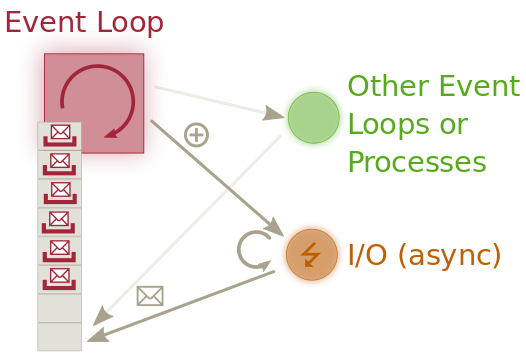
\includegraphics[scale=0.5]{./img/eventloop.png}
\end{array}$
\end{center}
\caption[Event-Loop]{Grafické znázornění Event-Loop}
\end{figure}

\subsection{Balíčkovací systém NPM}
Zejména v~posledních letech začali být velmi populární balíčkovací systémy pro různé programovací jazyky nebo frameworky inspirované balíčkovacími systémy z~operačního systému Linux respektive z~různých distribucí OS Linux. Vše začal jazyk Ruby a~především framework Ruby On Rails se~systémem tzv. Gemů. PHP dostalo balíčkovací systémy composer (aplikační moduly) a~pecl (systémové moduly). Python má pip atd,... NodeJS obsahuje svůj vlastní balíčkovací systém NPM (Node Package Manager). Disponuje velmi jenoduchům ovládáním a~přináší programátorů řešení závislostí jejich aplikací a~knihoven napříč operačními systémy.\cite{NodeJS}\\

Důležitým prvkem je konfigurační soubor \it{package.json}, obsahuje nejen informace o~závislostech programu, ale také třeba autora, verzi, popis, repozitář a~mnoho dalších údajů využívaných dalšími moduly aplikace.\\

Ukázkový package.json
     \begin{codeframe} 
      \begin{Verbatim}{frame=single}
{
  "name": "moje-aplikace",
  "version": "0.0.1",
  "dependencies": {
    "coffee-script": "^1.7.1",
    "express": "3.5.1",
    "mongoose": "^3.8.8",
  },
  "devDependencies": {
    "angular": "=1.2.16",
    "angular-ui-router": "^0.2.10",
  },
  "engines": {
    "node": ">=0.8.0"
  },
  "browserify": {
    "transform": [
      "coffeeify",
      "brfs",
      "envify"
    ]
  },
  "scripts": {
    "dev": "gulp dev",
    "prod": "gulp prod"
  }
}
\end{Verbatim} 
    \end{codeframe}
Ze souboru můžeme vyčíst, že jméno aplikace je "moje-aplikace", že se nachází ve verzi "0.0.1", jejími závislostmi jsou "coffee-script,express a mongoose", vývojovými závislostmi pak "angular a angular-ui-router", k běhu potřebuje nodejs ve verzi 0.8.0 a~vyšší. Modul browserify používá transformace: "coffeeify, brfs a envify" a~na závěr jsou dekplarované scripty.


NPM také obsahuje interaktivný shell pro vytváření nových projektů, který vytvoří package.json za uživatele. Nově instalované moduly jsou při přidání přepínače \it{--save} nebo \it{--save-dev} přidávány také automaticky.\\

Základní příkazy:
\begin{description}
 \item[install] nainstaluje balíčky v package.json
 \item[install <balíček>] nainstaluje balíček
 \item[update] aktualizuje balíčky v package.json
 \item[search] vyhledávání balíčků
\end{description}

\subsection{ExpressJS}
ExpressJS je webový framework inspirovaný webovým frameworkem Synatra napsaným v ruby. Jedná se o~malý flexibilní a~robustní framework pro pro psaní single-page, multi-page a hybrodných stránek postavený na NodeJS.\cite{expressjs}
\begin{figure}[h]
\begin{center}$
\begin{array}{c}

\includegraphics[scale=0.5]{./img/express.png}
\end{array}$
\end{center}
\caption[Logo ExpressJS]{Logo ExpressJS}
\end{figure}

Express je ve stylu Synatra designován jako velmi jednoduchý a~obsahuje tak velmi malé množství funkcí, které se rozšiřuje pluginy a~knihovnami. Express tak umí především zpracovávat routy (url cesty), html požádavky (POST,GET,PUT,PATCH,OPTION) a~tělo requestů. Umí také zpracovávat a~poskytovat statické soubory a cookies.\cite{expressjs}\\

Ukázka velmi jednoduché express aplikace:
     \begin{codeframe} 
      \begin{Verbatim}{frame=single}
express = require 'express'
server = express()
port = 3000;

app.get "/", (req, res, next)->
  res.render "views/root"

app.get "/hello", (req, res, next) ->
  res.send('world')

app.listen port, ->
  console.log("Listening on #{port})
\end{Verbatim} 
    \end{codeframe}
Pos spuštění kódu se vytvoří http server na portu 3000, který má dvě definované routy: \b{/} - root aplikace vrátí soubor \it{views/root.html} a \b{/hello}, který vrátí řetězec "world".

\subsection{Mongoose ODM}
V posledních letech se stali velmi populární ORM frameworky nad MySQL databází jako je Doctrine. Pro MongoDB databázi v~prostředí NodeJS je velmi populární ODM framework Mongoose. V~MongoDB databázi neexistuje schéma jako je tomu u~SQL databází jako je MySQL. Mongoose přináší podporu pro databázové schémata validaci a~virtuální položky funkce pro práci se schématem a~rozsiřitelné API. \\

Jednoduché schéma v Mongoose:

     \begin{codeframe} 
      \begin{Verbatim}{frame=single}
mongoose = require 'mongoose'
Schema = mongoose.Schema

User = new Schema
  email:
    type: String
    required: true
    unique: true
    index: true
  name:
    type:String
    required:false
  address:
    city: String
    state: String
  buyed_books:
    [
      type: Schema.Types.ObjectId
      ref: "Book"
    ]
  updated_at:
    type:Date
    default: Date.now
  created_at:
    type:Date
    default: Date.now

module.exports = mongoose.model 'User', User
\end{Verbatim} 
    \end{codeframe}
Schéma obsahuje teké definované typy objektů a~jejich validaci. Konkrétně toto schéma uživatele má objekty: \b{email-} indexovaný, unikátní a~povinný, \b{name-} jméno-řetězec, \b{address-} který má vnořený objekt, který~obsahuje město a~stát, \b{buyed\_books-}pole referencí na knihy, které~uživatel koupil, \b{update\_at,created\_at-}data vytvoření a~poslední úpravy uživatele.

\subsection{HapiJS (HTTP API)}
Pro nodeJS existuje opravdu obrovské množství nejrůznějších frameworků. Framework použitý pro tvorbu tohoto projektu se jmenuje \b{HapiJS} \href{http://spumko.github.io/}{http://spumko.github.io/}.\\

Jednáse o~jednoduše konfigurovatelný framework s~podporou validací, cachování, autentizace atd. Zaměřuje se na psaní znovupoužitelného aplikačního kódu a~eliminuje zdlouhavé vytváření infrastruktury.\cite{hapiJS}\\

Ukázka vytvoření základního serveru s~jednou routou "/":

     \begin{codeframe} 
      \begin{Verbatim}{frame=single}
Hapi = require("hapi")

# Vytvoří http server
server = Hapi.createServer("localhost", 8000)

# Root route vrátí text "hello word"
server.route
  method: "GET"
  path: "/"
  config:
    handler: (request, reply) ->
      reply "hello word"

# Spustí http server
server.start ->
  console.log "Server started at port " + server.info.port
  return
\end{Verbatim} 
    \end{codeframe}

Hapi jak už bylo řečeno Hapi obsahuje spoustu build-in\footnote{Build-in - Označuje funkcionalitu, která je již součástí} funkcionality, která ulehčuje práci programátorů a~usnadňuje rozdělení a~znovupoužitelnost aplikace. Jsou jimi např.:\\

\subsubsection{Error handler}
Hapi obsahuje build-in funkci pro vyvolání chybových odpovědí pomocí modulu "boom". Následující vyvolá HTTP vyjímku se stavovým kódem "499" a~zprávou špatný dotaz.\cite{hapiJSDOC}

     \begin{codeframe} 
      \begin{Verbatim}{frame=single}
(request, reply) ->
  error = Hapi.error.badRequest("Špatný dotaz")
  error.output.statusCode = 499
  error.reformat()
  error.output.payload.custom = "abc_123"
  reply error
\end{Verbatim} 
    \end{codeframe}

\subsubsection{Pack}
Pack je funkcionalita, která umožňuje sdružování množství serverů do jedné logické jednotky. Tokový pack může sdruzovat několik serverů, které~mohou mít vlastní pluginy.\cite{hapiJSDOC}
     \begin{codeframe} 
      \begin{Verbatim}{frame=single}
Hapi = require("hapi")
pack = new Hapi.Pack()
pack.server 8000,
  labels: ["web"]

pack.server 8001,
  labels: ["admin"]
\end{Verbatim} 
    \end{codeframe}
Vytvoření dvou serverů "web" a "admin"

\subsubsection{Composer}
Composer slouží k~jednoduché konfiguraci Packu v~jenom jediném objektu včetně registrace pluginů\cite{hapiJSDOC}.
     \begin{codeframe} 
      \begin{Verbatim}{frame=single}
Hapi = require("hapi")
manifest =
  pack:
    cache: "catbox-memory"
  servers: [
    {
      port: 8000
      options:
        labels: ["web"]
    }
    {
      host: "localhost"
      port: 8001
      options:
        labels: ["admin"]
    }
  ]
  plugins:
    yar:
      cookieOptions:
        password: "secret"
composer = new Hapi.Composer(manifest)
\end{Verbatim} 
    \end{codeframe}
Vytvoření dvou serverů "web" a "admin" s~pluginem yar a~jeho nastavením.

\subsubsection{Plugin}
Plugin je asi to nejzajímavější co HapiJS přináší. Plugin dokáže nést nějakou funkcionalitu, jako je zpracování requestu, nebo vlastní logiku. Plugin pomáhá rozdělit aplikaci na malé čášti, které mohou mít vlastní routy, závislosti, modely, logiku apd,... V různých kombinacích tak aby byli použitelné ve různých prostředích (development, testování, produkce).\cite{hapiJSDOC}
\begin{codeframe}
  \begin{Verbatim}
Hoek = require("hoek")
internals = defaults:
  version: "/version"

internals.version = 0.1
exports.register = (plugin, options, next) ->
  settings = Hoek.applyToDefaults(internals.defaults, options)
  if settings.version
    plugin.route
      method: "GET"
      path: settings.version
      handler: (request, reply) ->
        reply internals.version
        return

  listPlugins = (server) ->
    plugins = []
    Object.keys(server.pack.list).forEach (name) ->
      item = server.pack.list[name]
      plugins.push
        name: item.name
        version: item.version
    plugins

  plugin.expose "plugins", listPlugins
  next()
\end{Verbatim}
  \end{codeframe}
Jednoduchá ukázka pluginu, který přidává routu "/version", která vrátí jeho verzi a~metodu listPlugins, která vypíše všechny pluginy.

\subsubsection{Cyklus requestu}
Každý příchozí request musí projít sérií předefinovaných kroků spolu s~dalšími kroky přidanými programátorem.
Each incoming request passes through a pre-defined set of steps, along with optional extensions\cite{hapiJSDOC}:
\begin{description}
\item['onRequest'] do objektu procházejícího tímto budem jsou přidány metody "request.setUrl(url)" a~"request.setMethod(verb)". Tyto metody mají vliv na routování a~mohou být využity pro přepsání pravidel routování. Router není ještě inicializován. Jedná se o~bod, kterému můžeme přidat vlastní metody a~změnit tak chování aplikace.
\item[Procházení rout pomocí request path]
\item[Parsování cookies]
\item['onPreAuth'] další rozšiřující, bod, kterým je možné aplikaci rozšířit
\item[Authenticate request]
\item[Čtení a parsování payload]
\item[Authenticate request payload]
\item['onPostAuth'] další rozšiřující, bod, kterým je možné aplikaci rozšířit
\item[Validace parametrů cesty]
\item[Zpracování query (JSONP)]
\item[Validace query]
\item[Validace payload]
\item['onPreHandler'] další rozšiřující, bod, kterým je možné aplikaci rozšířit
\item[Přednastavení routeru]
\item[Router]
\item['onPostHandler'] další rozšiřující, bod, kterým je možné aplikaci rozšířit. V tomto kroce může býť modifikována odpověď serveru.
\item[Validace payload odpovědi]
\item['onPreResponse'] další rozšiřující, bod, kterým je možné aplikaci rozšířit
\item[Odeslání odpovědi] (může vyvolat 'internalError')
\item[Emits 'response' event]
\item[Emits 'tail' event]
\end{description}


\section{\upc{MongoDB}}
\begin{figure}[h]
\begin{center}$
\begin{array}{c}

\includegraphics[scale=0.5]{./img/mongodb.png}
\end{array}$
\end{center}
\caption[Logo MongoDB]{Logo MongoDB}
\end{figure}
MongoDB je dokumentová NoSQL databáze s~dokumenty ve formatu json a~dynamickým schématem. Počátek jejího vývoje spadá do roku 2007 a~je vyvýjena společností 10gen, momentálně se nachází ve verzi 2.6.\\

MongoDB funguje jako klasický databázový server, ke kterému se klienty připojují přes síť (obvykle na portu 27017) a~komunikují s~ním speciálním protokolem (ovšem na portu 28017 najdete jednoduché HTTP rozhraní). Součástí instalace je knihovna pro C++, jako součásti projektu jsou ale vyvíjeny a~podporovány i~knihovny pro Javu, Python, Ruby, PHP a~další jazyky.\\

MongoDB navíc obsahuje mnoho pokročilích funkcí, jako je replikace databáze, balancování zátěže (load balancing), ukládání souborů (file storage), indexace a~další,... \\

Základním rozhraním pro MongoDB je javascriptová konzole, kterou lze spustit příkazem \b{mongo}.\cite{abcLinuxuSerialMongo}

Vkládání záznamů:
     \begin{codeframe} 
      \begin{Verbatim}{frame=single}
db.users.insert(
  {
    name: "Franta",
    email: "franta@franta.cz", 
    address:{
      city:"zlín"
    }
  })
\end{Verbatim} 
    \end{codeframe}
Vytvoří záznam v~kolekci uživatelé se jménem "Franta", e-mailem "franta@franta.cz" a~adresou "zlín".
   
Hlednání:   
     \begin{codeframe} 
      \begin{Verbatim}{frame=single}
db.users.find()
#vrátí všechny záznamy

db.bands.find({name:"Franta"})
#vrátí záznamy se jménem Franta

db.bands.find({name: /^Fra.*/})
#regulérní výrazy v~dotazech
#vrátí všechny záznamy začínajích na Fra
\end{Verbatim} 
    \end{codeframe}

Update:
     \begin{codeframe} 
      \begin{Verbatim}{frame=single}
db.users.update(
  {
    _id: ObjectId("4b76ef5780b71853fe6c89b6")
  }, {
    $set: {
      email: "franta2@seznam.cz"
    }
  })  
\end{Verbatim} 
    \end{codeframe}
provede update uživatele id 4b76ef5780b71853fe6c89b6 a~zmnění jeho email na "franta2@seznam.cz"

Mazání:

     \begin{codeframe} 
      \begin{Verbatim}{frame=single}
db.users.remove({name: "Franta"})
\end{Verbatim} 
    \end{codeframe}
smaže všechny uživatele se jménem "Franta"

reference:
     \begin{codeframe} 
      \begin{Verbatim}{frame=single}
#přidáme uživateli koupenou knihu
db.users.update(
  {
    _id: ObjectId("4b76ef5780b71853fe6c89b6")
  }, {
    $push: {
      buyed_books: new DBRef("books", ObjectId("4b7b1d6bb345126b62fb2230"))
    }
  })

#vyhledáme uživatele
db.users.findOne({_id: ObjectId("4b76ef5780b71853fe6c89b6")})
#výstup
{
  "_id" : ObjectId("4b76ef5780b71853fe6c89b6"),
  "name":"Franta",
  "email":"franta@seznam.cz",
  "books" : [
          {
                  "$ref" : "books",
                  "$id" : ObjectId("4b7b1d6bb345126b62fb2230")
          }
  ],
  "address":{
    "city":"zlín"
  }
}
#získáme knihy uživatele
db.users.findOne({_id: ObjectId("4b76ef5780b71853fe6c89b6")}).books.fetch()
#výstup je stejný jako v přechozím případě jen v poli books
# se místo reference oběví objekt konkrétní khiny.
\end{Verbatim} 
    \end{codeframe}

\section{\upc{AngularJS}}
\begin{figure}[h]
\begin{center}$
\begin{array}{c}

\includegraphics[scale=0.5]{./img/angularjs.png}
\end{array}$
\end{center}
\caption[Logo AngularJS]{Logo AngularJS}
\end{figure}

Anglický originál popisu angularJS z repozitáře na portále github.com


\it{AngularJS lets you write client-side web applications as if you had a smarter browser. It lets you use good old HTML (or HAML, Jade and friends!) as your template language and lets you extend HTML’s syntax to express your application’s components clearly and succinctly. It automatically synchronizes data from your UI (view) with your JavaScript objects (model) through 2-way data binding. To help you structure your application better and make it easy to test, AngularJS teaches the browser how to do dependency injection and inversion of control. Oh yeah and it also helps with server-side communication, taming async callbacks with promises and deferreds; and makes client-side navigation and deeplinking with hashbang urls or HTML5 pushState a piece of cake. The best of all: it makes development fun!}\cite{angularGITHUB}\\

Překlad:

\it{AngularJS vám umožní vytvářet tenké klientské aplikace, jakobyste měli chytřejší prohlížeč. Přitom můžete používat staré známé HTML (HAML, JADE a~podobné) jako šablonovací systém a~rozšířit jeho syntaxy tak aby komponenty vyjadřovali aplikaci jasně a~stručně. Automaticky synchornizuje data v~uživatelském rozhraní s~vaším javascriptovým modelem, pomocí obousměrné datové vazby. Abyste mohli strukturovat vaši aplikaci lépe a~udělali ji snáze testovatelnou, AngularJS učí váš prohlížeč jak na devendency injection a~inversion of~control. A abych nezapomněl také vám pomůže s~komunikací se serverem, pomůže vám zkrotit asynchroní callbacky, promises a~deferreds; a~také dělá navigaci v~prohlížeči, pomocí deeplinking s~hashbang url nebo html5 pushState snadnou věcí. A to nejlepší na konec: dělá vývoj webových aplikací zábavou.}\cite{angularGITHUB}\\

\subsection{Struktura}
Struktura kódu aplikace by měla mít nějaká pravidla, tak aby se v~kódu vyznam i~někdo jiný než autor samotný. Proto napříkal google poskytuje online doporučenou strukturu kódu pro aplikace napsané v~AngularJS. Online verze je dostupná na adrese: \href{https://google-styleguide.googlecode.com/svn/trunk/angularjs-google-style.html}{https://google-styleguide.googlecode.com/svn/trunk/angularjs-google-style.html}
\it{Vzhledem k tomu,že se jedná o~obsáhlejší dokument nebude nijak komentován. Ale struktura aplikace je z~větší části ovlivněna právě tímto návrhem.}\\

Co se týče struktury adresářové, existuje zde několik návrhů, které jsou určeny pro různě velké aplikace.\\

Velmi jednoduchá aplikace v~AngularJS vypadá nějak takto:
     \begin{codeframe} 
      \begin{Verbatim}{frame=single}
css/
img/
js/
  app.js
  controllers.js
  directives.js
  filters.js
  services.js
lib/
partials/
\end{Verbatim} 
    \end{codeframe}
Vše je rozděleno do několika javascriptových souborů, které reprezentují jednotlivé moduly AngularJS, je to o~něco málo lepší, než jednosouborové aplikace tak jak to dělá velké množství uživatelů jQuery, ale jednotlivé soubory nereprezentují konkrétní funkcionalitu, takže se v projektu hůře orientuje.\cite{angularJSFolders}\\

Tento problém řeší rozdělení jednotlivých modulů do několika sub-modulů, které již reprezentují svoji funkcionalitu.
     \begin{codeframe} 
      \begin{Verbatim}{frame=single}
controllers/
  LoginController.js
  RegistrationController.js
  ProductDetailController.js
  SearchResultsController.js
common/
  cartDirective.js
  productFilter.js
models/
  CartModel.js
  ProductModel.js
  SearchResultsModel.js
  UserModel.js
services/
  CartService.js
  UserService.js
  ProductService.js
\end{Verbatim} 
    \end{codeframe}

V~případě, že vytvářím, větší aplikaci, stane se pro mě toto schéma také nedostatečným, protože ve větších aplikacích už je většinou třeba shlukovat veškeré části dané funkcionality u~sebe, takže ještě je třeba strukturu ještě přeskupit.\\
     \begin{codeframe} 
      \begin{Verbatim}{frame=single}
cart/
  index.less
  CartModel.js
  CartService.js
common/
  cartDirective.js
  productFilter.js
product/
  search/
    SearchResultsController.js
    SearchResultsModel.js
  ProductDetailController.js
  ProductModel.js
  ProductService.js
  index.less
  show.html
user/
  show.html
  edit.html
  index.less
  LoginController.js
  RegistrationController.js
  UserModel.js
  UserService.js
\end{Verbatim} 
    \end{codeframe}

\subsection{Router}
Router je další důležitá přednost AngularJS, jak už bylo v úvodu zmíněno routování umožňuje přepínat mezi url hashangem a~html5.pushState. Router v AngularJS je navíc modulem, který lze vyměnit takže můžeme místo něj použít třeba ui-router, který jeden z~nejpoužívanějších modulů pro AngularJS. Oproti angular-routeru je ui-router stavový, takže každá změna ui může být reprezentována svým stanem, který můze být jednoduše vnořen a~výsledkem je pak přehledná hierarchie routeru a~url.\\

Ukázka jednoduché routeru v~modulu angular-router
     \begin{codeframe} 
      \begin{Verbatim}{frame=single}
phonecatApp.config [
  "$routeProvider"
  ($routeProvider) ->
    $routeProvider.when("/phones",
      templateUrl: "partials/phone-list.html"
      controller: "PhoneListCtrl"
    ).when("/phones/:phoneId",
      templateUrl: "partials/phone-detail.html"
      controller: "PhoneDetailCtrl"
    ).otherwise redirectTo: "/phones"
]
\end{Verbatim} 
    \end{codeframe}
Zde jsou nastaveny routy \b{/phones} , která má controller: "PhoneListCtrl" a~template: partials/phone-list.html a~\b{/phones/:id}, která slouží pro získání jednoho telefonu. Pokud není routa v~seznamu, je přesměrováno na routu "/phones"

Ukázka ui-router
     \begin{codeframe} 
      \begin{Verbatim}{frame=single}
phonecatApp.config [
  "$stateProvider, $urlRouterProvider",
  ($stateProvider, $urlRouterProvider) ->
    $urlRouterProvider.otherwise "/phones"
    $stateProvider.state("phones",
      url: "/phones"
      templateUrl: "partials/phones-list.html"
    ).state("phones.one",
      url: "/:id"
      templateUrl: "partials/phone-detail.list.html"
      controller: "PhoneDetailCtrl"
    )
]
\end{Verbatim} 
    \end{codeframe}
Stejný případ jako u normálního angular-routery, ale tentokrát s~ui-routerem. Z ukázky je vidět, že stavy v~ui-routeru, jsou hierarchycké a lépe se v~nich orientuje.\\

\subsection{Scope}
Scope je základním stavebním kamenen AngularJS aplikací. Scope reprezentují model aplikace, jsou také místem kde dochází k~vyhodnocení výrazů $\{\{ \}\}$, definujeme zde bussines logic aplikace metody našich controllerů a~vlastnosti views. Scope svazuje controller a~view, těsně před tím než se view zobrazí uživateli, je template prolinkován se scope a~DOM nastaven tak aby o~všech změnách informaval AngularJS.\cite{ngBOOK}\\

Scope také tvoří hierarchické struktury, téměř každá directiva vytváří vlastní scope.

\subsection{Controller}
Controller je funkcí, která přidává další funkcionalitu scope a~je volán při jejím vytvoření.\cite{ngBOOK}

Ukázka jednoduchého kontrolleru
     \begin{codeframe} 
      \begin{Verbatim}{frame=single}
#VIEW:
<div ng-app="myApp">
  <div ng-controller="Controller" ng-init="init()">
    Jmeno: {{user}}
  </div>
</div>

#CONTROLLER:
app.controller "Controller", ["$scope","api",($scope,api) ->
  $scope.user = ""
  $scope.init =->
    $scope.user = api.getUser()

#výsledek
Jmeno: Franta
\end{Verbatim} 
    \end{codeframe}
Jenoduché vypsání jména uživate, které je získáno z~factory "api" funkcí "getUser()".

\subsection{Directive}
Directivy jsou místem kde je v~AngularJS zpracováván DOM. AngularJS je plný directiv\footnote{seznam build-in directiv pro AngularJS je~k~dispozici v~dokumentaci: \href{https://docs.angularjs.org/api/ng/directive}{https://docs.angularjs.org/api/ng/directive}}, už pro vyvoření AngularJS aplikace je třeba využít directivu \it{ng-app}.\cite{ngBOOK}\\

Zpracování directivy má 3~fáze, \it{compile, link a controller}, které jsou vykonány v~tomto pořadí. Directivu můžeme bindovat na DOM element několik způsoby\cite{ngBOOK}:
\begin{description}
\item[E] Element <mojeDirectiva></directiva>
\item[A] Atribut <div mojeDirectiva=""~></div>
\item[C] Třída <div class="mojeDirectiva"~></div>
\item[M] Komentář <!-- directive: mojeDirectiva exp -->
 \end{description}

 Diractiva může mít vlastní HTML template, vlastní scope,controller, můžeme určit prioritu jejího vykonání, apd... Ve všech ohledech je directiva velmi dobře znovuvyužitelný komponent aplikace.\cite{ngBOOK}\\

Ukázka directivy:
     \begin{codeframe} 
      \begin{Verbatim}{frame=single}
app.directive "loading",->
  restrict: "E"
  replace:true
  scope:{}
  link: (scope) ->
    scope.$on "LOADING",->
      scope.loading=true
    scope.$on "LOADING_END",->
      scope.loading=false

  template:'<div class="loading" ng-if="loading"></div>'

VIEW:
<loading></loading>
\end{Verbatim} 
    \end{codeframe}
Directivatu "loading" je možné "bindovat" na DOM element s~názvem "loading". Pokud directiva obdrží "\$broadcast" "LOADING", zobrazí se DOM element s~načítáním a~pokud obdrží "\$broadcast" LOADING\_END skryje načítání.\cite{ngBOOK}

\subsection{Factory}
Obecně lze říci, že service providery, jakým je i~factory, jsou k~tomu aby pro všechny controllery aplikace poskytovali stejné metody a~data, po dobu exsitence aplikace.\\

Jedná se vždy o~objekt singleton, který je instancován jednou za život aplikace pomocí \it{\$injector} service.\cite{ngBOOK}\\

Časté je použití factory jako helper pro komunikaci s~backendem aplikace, localStorage, cookieStorage apd,…\\

Ukázka jednoduché factory pro generování náhodných čísel:
     \begin{codeframe} 
      \begin{Verbatim}{frame=single}
app.factory "random", ->
  randomNumber:->
    Math.floor(Math.random())
  randomNumberBetween:(min,max)->
    Math.random() * (max - min) + min
  randomFromArray:(array)->
    array[Math.floor(Math.random() * array.length)]
\end{Verbatim} 
    \end{codeframe}
Factory v~příkladu je spíše takový "hellper"\footnote{hellper - pomocná funkce,třída nebo knihovna}. Má tři metody, které vrací buď náhodné číslo, náhodné číslo mezi dvěma hodnotami nebo~náhodný prvek pole.

\subsection{Filter}
Filter jak už název napovídá je určen pro filtraci dat. Je možné ho použít formou service v~controlleru nebo přímo ve view pomocí "roury" \it{\{\{ data | filter \}\}}. AngularJS má několik buildin filtrů jako je \it{date, lowercase, ...}.\cite{ngBOOK}

Ale je možné si nadefinovat také vlastní filtry, následující filter děla jednoduchou věc a~to, že~drží danný počet míst čísla tak, že~před číslo doplňuje nuly:
     \begin{codeframe} 
      \begin{Verbatim}{frame=single}
app.filter "numberpad", ->
  (input, places) ->
    out = ""
    if places
      placesLength = parseInt(places, 10)
      inputLength = input.toString().length
      i = 0

      while i < (placesLength - inputLength)
        out = "0" + out
        i++
      out = out + input
    out
#použití:
<div>{{minutes|numberpad:2}}</div>

#výsledek
$scope.minutes = 1
<div>01</div>
\end{Verbatim} 
    \end{codeframe}

\subsection{Animace}
Od verze 1.2 disponuje AngularJS přepracovanými animacemi v~samostatném modulu \it{angular-animate}. Definovat animace je díky tomuto modulu velmi jednoduché snadno pochopitelné a~velmi příjemné. K~animacím jsou používány běžné css animace, které jsou definovány pomocí css selectorů. \cite{angularAnimation}\\

Většina AngularJS directivy jako \it{ngRepeat,ngShow, apd...} má vlastní hooky, které jsou spouštěny v určitých fázích cyklu directivy.\cite{ngBOOK}\\

Ukázka ng-hide animace:
\begin{codeframe}
  \begin{verbatim}
#DOM
<div class="anim" ng-hide="checked" ng-click="checked=false">Hide<div>

#CSS
.anim.ng-hide-add, .anim.ng-hide-remove {
  transition:all linear 0.5s;
  display:block!important;
}

.anim.ng-hide-add.ng-hide-add-active,
.anim.ng-hide-remove {
  opacity:0;
}

.anim.ng-hide-add,
.anim.ng-hide-remove.ng-hide-remove-active {
  opacity:1;
}
  \end{verbatim}
\end{codeframe}
tato animeca je určena pro directivu "ngShow". Z~kódu lze vyčíst, že~při přidaní a~odebrání elementu, repspektive při přidání třídy "ng-hide-add" a "ng-hide-remove", se~provede lineární animace trvající 0.5s a~po tuto dobu bude trvat přechod z~průhlednosti 1 do průhlednosti 0. Tak může být docíleno zmizení jakéhokoliv DOM elementu.\cite{ngBOOK}

Další informace jak vytvářet vlastní animace je možné se dozvědět v~dokumentaci projektu: \href{https://docs.angularjs.org/guide/animations}{https://docs.angularjs.org/guide/animations}\\

\section{\upc{LESS}}
\begin{figure}[h]
\begin{center}$
\begin{array}{c}

\includegraphics[scale=0.5]{./img/less.png}
\end{array}$
\end{center}
\caption[Logo Less]{Logo Less}
\end{figure}
LESS je pre-processorem CSS stylů a~jeho účelem je rozšířit funkconalitu CSS jazyka. CSS je velmi jednoduché a~nanabízí dynamičnost, která je dnes velmi potřebná a~je často vyžadována projektem samotným. Právě k tomuto účelu se používá pre-procesor. Zejmnéna jsou v~dnešní době používány následující pre-procesory \it{LESS, SASS a Stylus}. Ve své podstatě jsou si podobné a~nabízí i~podobnou funkcionalitu. Všechny mají stejné vnořené selectory, svůj systém promněnných, cykly, mixin, funkce a~mnoho dalších nástrojů usnadňujících práci developerům.\cite{lesscss}\\

jednoduchá ukázka less:
\begin{codeframe}
  \begin{verbatim}
#proměnná
@color: #f938ab;

#mixin
.box-shadow(@style, @c) when (iscolor(@c)) {
  box-shadow:         @style @c;
}
#mixin
.box-shadow(@style, @alpha: 50%) when (isnumber(@alpha)) {
  .box-shadow(@style, rgba(0, 0, 0, @alpha));
}

.box {
  color: saturate(@color, 5%);
  #vnořený selector
  div { .box-shadow(0 0 5px, 30%) }
}

#výsledek
.box {
  color: #fe33ac;
 }
.box div {
  box-shadow: 0 0 5px rgba(0, 0, 0, 0.3);
}
  \end{verbatim}
\end{codeframe}

\subsection{Twitter bootsrap}
TODO:

\subsection{LessHat}
TODO:


\section{\upc{JADE}}
\begin{figure}[h]
\begin{center}$
\begin{array}{c}

\includegraphics[scale=0.5]{./img/jade.png}
\end{array}$
\end{center}
\caption[Logo Jade]{Logo Jade}
\end{figure}
Jade je velmi podobý CoffeeScriptu nebo YAMLu, jedná se o~template engine velmi často používaný v~NodeJS aplikacích. Zjednodušuje syntaxy HTML jazyka tím, že odstraňuje párovost HTML tagů a~hierarchii elementů určuje indentace řádků.\\

Jednoduchá ukázka HTMl dokumentu napsaného v~JADE mluví za vše a~každý kdo zná HTML, zná i~jade:
\begin{codeframe}
  \begin{verbatim}
#JADE
doctype html
html(lang="en")
  head
    title= pageTitle
    script(type='text/javascript').
      if (foo) {
         bar(1 + 5)
      }
  body
    h1 Jade - node template engine
    #container.col
      if youAreUsingJade
        p You are amazing
      else
        p Get on it!
      p.
        Jade is a terse and simple
        templating language with a
        strong focus on performance
        and powerful features.

#HTML
<!DOCTYPE html>
<html lang="en">
  <head>
    <title>Jade</title>
    <script type="text/javascript">
      if (foo) {
        bar(1 + 5)
      }
    </script>
  </head>
  <body>
    <h1>Jade - node template engine</h1>
    <div id="container" class="col">
      <p>You are amazing</p>
      <p>Jade is a terse and simple
         templating language with a
         strong focus on performance
         and powerful features.</p>
    </div>
  </body>
</html>
  \end{verbatim}
\end{codeframe}\cite{jade}

\section{\upc{Bower}}
\begin{figure}[h]
\begin{center}$
\begin{array}{c}

\includegraphics[scale=0.5]{./img/bower.png}
\end{array}$
\end{center}
\caption[Logo Bower]{Logo Bower}
\end{figure}
Bower je velmi podobný NodeJS balíčkovacímu systému NPM. Bower, ale slouží k~určení balíčkovýčh závislostí pro různé javascriptové knihovny, jako je AngulaJS, JQuery, apd,... Usnadňuje především plnění závislostí na externích javascriptových knihovnách a~odlehčuje repozitářům, protože odpadá verzování knihovních závislostí a~zůstávají pouze reference na ně, které stáhne bower při buildu aplikace.\cite{bower}\\

Bower disponuje stejně jako NPM interaktivním scriptem pro vytváření projektů a~má podobnou comand-line syntaxy:\\
\begin{description}
 \item[install] nainstaluje balíčky v bower.json
 \item[install <balíček>] nainstaluje balíček
 \item[update] aktualizuje balíčky v bower.json
 \item[search] vyhledávání balíčků
\end{description}

\section{\upc{GulpJS}}
\begin{figure}[h]
\begin{center}$
\begin{array}{c}

\includegraphics[scale=0.5]{./img/gulp.png}
\end{array}$
\end{center}
\caption[Logo GulpJS]{Logo GulpJS}
\end{figure}
Gulp je task runner stejně jako známější Grunt, který je ve světě NodeJS aplikací zřejmně nejpoužívanějším task runnerem. Grunt a Gulp dělají ve~svě podstatě to samé, ale grunt má několik limitů, které překonává právě Gulp. Předvším se jedná o~návaznost úkolů. Grunt pracuje se soubory tak, že spustíme jeden taks např. překlad coffeescriptu, přeložené soubory uložíme, spustíme sloučení (concat) souborů, uložíme jinam spustíme uglifikaci apd,… Gulp používá datové streamy a~roury (pipes), kdy předává výstup jednoho úkolu duhému a~vše je tam v~jenom tasku. Konfigurace je tak mnohem jednodušší a~všechny úkoly probíhají asynchroně.\\

Ukázka gulp tasku pro zpracování LESS. Pro tento úkol by byly třeba alespoň 3 Grunt tasky.
\begin{codeframe}
  \begin{verbatim}
gulp.task('LESS_DEV', ["SPRITES_DEV"], function() {
    return gulp.src("./src/less/main.less")
        .pipe(debug({verbose: true}))
        .pipe(plumber())
        .pipe(less())
        .pipe(autoprefixer(confAutoPrefix))
        .pipe(gulp.dest("./build"))
        .pipe(livereload())
});
  \end{verbatim}
\end{codeframe}
Postupně jsou provedeny tyto kroky: \b{src} - vybere soubory a~vytvoří stream, \b{debug} - spustí ladění scriptu, \b{plumber}-zajistí, že~při chybě nedojde k~pádu gulpu, \b{less} - přeloží less zdrojové soubory, \b{autoprefixe} - vyřeší vendor prefixy prohlížečů na základě konfiguračního objektu, \b{dest} - uloží stream do souboru, \b{livereload} - obnoví livereload server.\cite{jade}

\section{\upc{Systém pro správu verzí git}}
Projekt git byl založen v~roce 2005 Linusem Torvaldsem, původně pro vývoj jádra Linuxu, a~jsou do něj vloženy zkušenosti, které Linus získal při vedení rozsáhlého projektu Linuxového jádra.~\cite{MailingListVznikGITu}\\

Git je zcela zdarma, open source, \b{distribuovaný systém pro správu verzí} navržený zvládnout vše od malých až~po~velmi rozsáhlé projekty s~rychlostí a~účinností. Každý klon Git je full-fledged (česky plně rozvinuté) úložiště s~kompletní historií a~veškerými schopnostmi sledování revizí a~nezávislostí na přístupu k~síti nebo centrálnímu serveru. Větvení (branching) a~slučování (merging) jsou rychlé a~snadné.~\cite{GITWEB} Velmi důležité je pak slovo distribuovaný, protože git neukládá každou změnu na centrální úložiště, ale~každý klon repozitáře obsahuje i~kompletní databázi změn projektu.

\subsection{Použití git v bakalářské práci}
Ke psaní této bakalářské práce byl zvolen sázecí systém \LaTeX, jednak pro jeho velmi kvalitní a~typograficky správný výstup, ale~i~protože je taková práce psána formou zdrojového kódu. Díky uložení zdrojového kódu do plain/text souboru je velmi snadné a~výhodné použít systému pro správu verzí. Systém git byl také použit pro správu verzí skriptů pro praktickou část \uv{LFS by BASH scripts}, které jsou uloženy také v~textových souborech.

\subsection[Základní příkazy a github]{Základní příkazy a sociální web github}
Ke správě jednoduchých a~malých projektů jako je např. tato bakalářská práce stačí umět opravdu jenom pár příkazů. A~díky webu github.com se stává správa malého projektu opravdu jednoduchou záležitostí.\\

\subsubsection{Nastavení gitu}
Základní nastavení gitu spočívá pouze v~nastavení Jména, Příjmení a~emailu. Pokud používáme git pouze lokálně a~nenahráváme data někam na server, bude nám to stačit a~můžeme již vytvořit repozitář.\\

Nastavení jména, příjmení a~emailu.~\cite{GIThelpNastaveni}
    \begin{codeframe}
      \begin{Verbatim}{frame=single}
git config --global user.name "Jméno Příjmení"
git config --global user.email "VášEmail@seznam.com"
\end{Verbatim} 
    \end{codeframe}
Pokud nahráváme data na server je třeba autentizace. K~účelu autentizace se často používá ssh klíč. Ten je možné vygenerovat následujícím způsobem~\cite{GIThelpNastaveni}
    \begin{codeframe}
      \begin{Verbatim}{frame=single}
ssh-keygen -t rsa -C "VášEmail@seznam.com"
\end{Verbatim} 
    \end{codeframe}
pak je třeba zadat dvakrát heslo pro otevírání klíče a~klíč je vygenerován.\\

Vygenerovaný klíč je k~nalezení v~domovském adresáři uživatele ve~složce \it{.ssh}, která obsahuje soubory \it{id\_rsa} a \it{id\_rsa.pub}. id\_rsa je váš privátní klíč a~id\_rsa.pub je klíč veřejný. Pro použití githubu je~třeba veřejný klíč nahrát do~nastavení na~webu \it{“Account Settings” > Click “SSH Public Keys” > Click “Add another public key”}. Také je potřebné nahrát do nastavení gitu bezpečnostní token githubu. Bezpečnostní token lze nalézt na webu \it{“Account Settings” > Click “Account Admin.”} položku API token, která obsahuje jakýsi HASH, je třeba vložit do~nastavení git na počítači.~\cite{GIThelpNastaveni}
    \begin{codeframe}
      \begin{Verbatim}{frame=single}
git config --global github.user uzivatelskeJmeno
git config --global github.token 0123456789yourf0123456789token
\end{Verbatim} 
    \end{codeframe}

\subsubsection{Vytvoření repozitáře a první commit}
Vytvoření repozitáře je velmi jednoduché a~skládá se ze dvou kroků: Vytvoření složky a~inicializace repozitáře.
    \begin{codeframe}
      \begin{Verbatim}{frame=single}
mkdir projekt
cd projekt
git init
\end{Verbatim} 
    \end{codeframe}
Změny v~repozitáři jsou reprezentovány commity. Commit je vytvořen přidáním jednoho nebo více souborů a~přidáním popisku. Jako první by měl projekt obsahovat soubor README.
    \begin{codeframe}
      \begin{Verbatim}{frame=single}
touch README
git add README
git commit -m 'přidáno README'
\end{Verbatim} 
    \end{codeframe}

Pokud chceme použít github, je třeba vytvořit repozitář na webu github. Po vyplnění názvu a~popisu repozitáře, github vypíše kroky nutné k~vytvoření repozitáře. Vypíše tedy, že je třeba vytvořit složku, inicializovat git, přidat první commit (nejčastěji soubor README), přidat adresu repozitáře na serveru github a~odeslání změn v~repozitáři.~\cite{GIThelpNastaveni}
    \begin{codeframe}
      \begin{Verbatim}{frame=single}
git remote add origin git@github.com:uzivatelskeJmeno/projekt.git
git push origin master
\end{Verbatim} 
    \end{codeframe}

\subsubsection{Správa repozitáře}
Každodenní správa repozitáře jednoduchého projektu je většinou o~přidávání commitů a~odesílání změn. Takže si většinou lze vystačit s~příkazy \it{add, rm, diff, commit, push a pull}. Ale git obsahuje také spoustu jiných užitečných funkcí, které usnadní správu i~malého projektu.\\

Commit není pouze přidávání souborů, ale~i~mazání a~změny v~souborech.
    \begin{codeframe}
      \begin{Verbatim}{frame=single}
git rm soubor #smaže soubor
git add #přidá soubor, pokud soubor změníme je třeba ho také přidat
git diff #ukáže změny v repozitáři
git commit #vytvoří commit
git push #odešle změny
git pull #stáhne změny ze serveru
\end{Verbatim} 
    \end{codeframe}

Jednou z~funkcí je \b{tag}. Tag vytvoří značku za~určeným commitem ke které se lze jednoduše vrátit. Je tedy užitečný pokud chce vytvořit např. release programu. commity a~jejich kódy si lze prohlédnout příkazem \it{git log}
    \begin{codeframe}
      \begin{Verbatim}{frame=single}
git tag v1.0 <kód commitu>
\end{Verbatim} 
    \end{codeframe}
K~tagu se lze jednoduše vrátit příkazem \it{checkout}. (příkaz \it{chekcout} také mění větve)
    \begin{codeframe}
      \begin{Verbatim}{frame=single}
git checkout v1.0
\end{Verbatim} 
    \end{codeframe}

Další funkcí, která je užitečná je branch (větev). Branch můžeme např. použít pokud se chystáme udělat změnu, o~které nevíme jistě, zda bude fungovat. Často je branch také k~oddělení prací uživatelů nebo částí projektu na kterých se pracuje.\\
Branch lze vytvořit příkazem
    \begin{codeframe}
      \begin{Verbatim}{frame=single}
git branch <název větve>
\end{Verbatim} 
    \end{codeframe}
Repozitář je automaticky přepnut na vytvořenou větev a~změny už se neprovádí v~hlavní větvi master, ale v~nové větvi. Vytváření commitů a~odesílání změn je pak normální. Nastane ale čas, kdy je třeba části větve nebo větev celou začlenit do větve hlavní. K~tomuto je několik příkazů: první z~nich je \it{rebase}, který stáhne změny z~hlavní větve a~aplikuje je před změny ve vytvořené větvi. Pokud v~projektu nevznikají změny souběžně v~hlavní větvi i~větvi nové, není rebase třeba. Změny aplikujeme pomocí změny větve zpět na master příkazem \it{checkout} a~odeslání změn z~vytvořené větve pomocí \it{pull}. (takto lze aplikovat změny mezi libovolnými větvemi)
    \begin{codeframe}
      \begin{Verbatim}{frame=single}
git checkout -f master
git pull . <název větve>
\end{Verbatim} 
    \end{codeframe}
Samozřejmě může nastat čas, kdy větev již není třeba a~chceme ji spojit s~hlavní větví nebo smazat.
    \begin{codeframe}
      \begin{Verbatim}{frame=single}
git merge <název větve> #spojí aktuální větev se zadanou
git branch -D <název větve> #smaže větev
\end{Verbatim} 
    \end{codeframe}
Pokud souběžně vznikají změny ve větvi hlavní i~nové větvi a~chceme provést příkazy jako \it{rebase, pull . <větev>} nebo \it{merge} mohou nastat konflikty ve změnách, které je třeba vyřešit (git některé konflikty řeší sám, ale nedokáže všechno). V takovém případě přepne git aktuální větev do speciálního režimu a~předá uživateli informace k~vyřešení těchto konfliktů.~\cite{GITmanualMerge}

\section{\upc{TeX}}
TODO:

%
%DALŠÍ
%
%browserify,lesshat,bootstrap

% \begin{codeframe}
%   \begin{verbatim}
%   <div class="check-element sample-show-hide" ng-show="checked" style="clear:both;">
%   \end{verbatim}
% \end{codeframe}

% \begin{figure}[h]
% \begin{center}$
% \begin{array}{c}
% 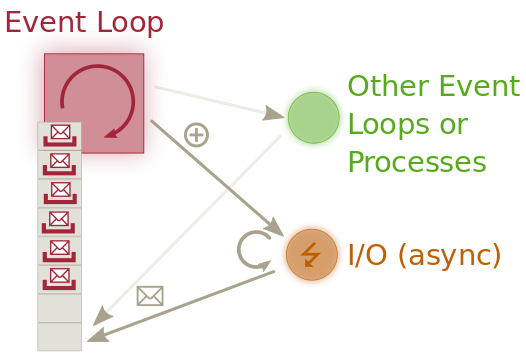
\includegraphics[scale=0.5]{./img/eventloop.png}
% \end{array}$
% \end{center}
% \caption[Grafické znázornění Event-Loop]{}
% \end{figure}


% \begin{description}
%  \item[ITEM] TEXT
%  \end{description}

% \subsubsection{subsub}

% \begin{itemize}
%  \item LFS učí uživatele, jak Linux funguje uvnitř.
% \end{itemize}
% \begin{enumerate}
% \item ITEM
% \end{enumerate}


% \nadpis{Remastersys}

% \nadpis{The Ubuntu Customisation Kit (UCK)}\\ \label{sec:UCK}
% \odkazNaKapitolu{sec:UCK}\\

% \begin{figure}[h]
% \begin{center}$
% \begin{array}{cc}
% 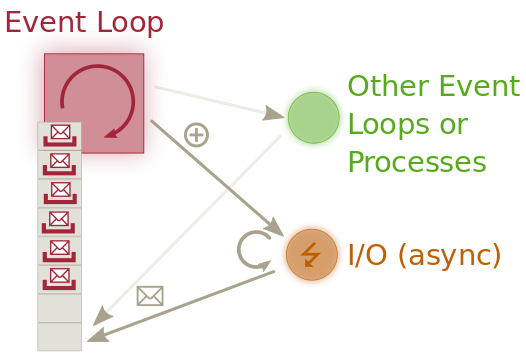
\includegraphics[scale=0.5]{./img/eventloop.png} &
% 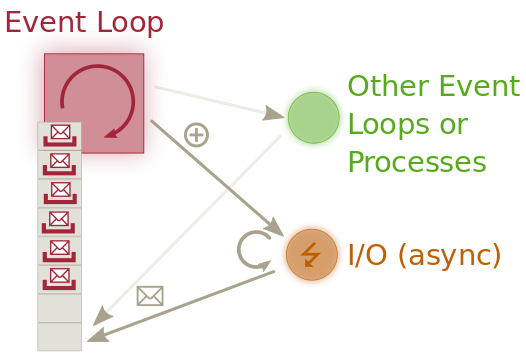
\includegraphics[scale=0.5]{./img/eventloop.png}
% \end{array}$
% \end{center}
% \caption[Webové rozhraní Instalinux, distribuce/časová zóna]{Webové rozhraní Instalinux, vlevo výběr distribuce, vpravo nastavení jazyka a~časové zóny}
% \end{figure}

\newpage

\vspace{4 mm}


%********************************* Analytická část ************************************
%\part{Analytická část}
%\sectionV{Nadpis}
%\subsection{Podnadpis}
%********************************* Projektová část ************************************
\part{Praktická část}
\section{\upc{Funkcionalita}}
Vzhledem k~modulárnosti a~škálovatelnosti aplikace lze na funkcionalitu nahlížet ze dvou pohledů.\\

Prvním je pohled z~hlediska modulárnosti aplikace jako takové a~její škálovatelnosti a~druhým pohled z~hlediska uživateského.\\

\subsection{Modulární aplikační funkcionalita}
V tomto pohledu, lze dělit funkcionalitu na Databázi \odkazNaKapitolu{sec:db}, Backend \odkazNaKapitolu{sec:backend} a~Frontend \odkazNaKapitolu{sec:frontend}.

\begin{figure}[h]
\begin{center}$
\begin{array}{c}
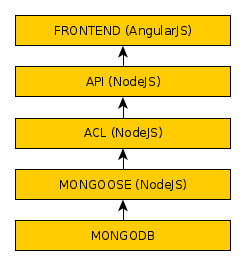
\includegraphics[scale=0.5]{./img/graph-structure.png}
\end{array}$
\end{center}
\caption[Diagram struktury aplikace]{Diagram struktury aplikace}
\end{figure}

Databázovou funkcionalitu obstarává MongoDB server, který je sám o~sobě škálovatelný a~může běžet na několika serverech.\\

Backend zajišťuje NodeJS aplikace, kterou lze dělit na části podle funkcionalit a~jednotlivé API mohou běžet na vlastních serverech. např. překlad TeX dokumentů může být uskutečňován na jiném serveru, fronend a~statické soubory mohou být distribuovány z~vlastního serveru, apd... Také zajišťuje integritu dat ukládaných do databáze a~restrikce uživatelského přístupu.\\

Frontend je pak rozdělen do několik single-page aplikací aby se klientovi, který přijde na e-shop nestahoval zbytečně např. také editor pro tvorbu knih, nebo části aplikace, které by neměly být přístupné. Frontend používá framework AngularJS a~jeho kód je plně vykonáván na klientské stanici, tedy v~prohlížeči. Data se stahují pomocí asynchroních javascriptových requestů.\\

\subsection{Uživatelská funkcionalita}
Uživatelská funkcionalita spočívá pouze na frontendu. Ten zajištůje, že uživatel vidí a~kupuje knihy.\\

Prakticky je frontend rozdělen to těchto single-page aplikací, kde každá znich poskytuje určitou funkcionalitu pro určité spektrum uživatelů.\\

\begin{description}
 \item[Store] jedná se o~jednoduchý uživatelsky přívětivý e-shop \odkazNaKapitolu{sec:store}
 \item[Create] rozhraní pro správu vlastních knih \odkazNaKapitolu{sec:create}
 \item[Edit] editor knih \odkazNaKapitolu{sec:create}
 \item[Finance]
 \item[Storage] sklady \odkazNaKapitolu{sec:storage}
 \item[Statistics] statistiky \odkazNaKapitolu{sec:stats}
 \item[Admin] administrace \odkazNaKapitolu{sec:admin}
\end{description}

jednotlivé aplikace budou rozebrány ve svých kapitolách.

\subsection{Proces schvalování knihy}
Podobně jako byl v teoretické části popsán proces schvalovaní knihy \odkazNaKapitolu{sec:schvalovani} probíhá proces schvalování i~v~aplikaci.

Proces schvalování má x kroků
....

Po schválení projektu může proběhnou akce vytvoření knihy z~projektu. Je standartně vytvořena kniha a~zní odkázáno na projekt, který jí předcházel. I~po publikaci je možné vytvořit opravy přímo pro již existující knihu. Nebo vydat další vydání ať už jako aktualizaci nebo novou knihu.

\section{\upc{Adresářová struktura projektu}}

statické soubory, do této složky probíhá build FrontEndu aplikace
\begin{codeframe}
  \begin{verbatim}
/assets
  \end{verbatim}
\end{codeframe}

konfigurační soubory backendu. Nachází se zde 3 soubory pro jednotlivá prosředí.\newline
\begin{codeframe}
  \begin{verbatim}
/config
  \end{verbatim}
\end{codeframe}
\it{appDev} - Development prostředí\newline
\it{appTest} - Testovací prostředí\newline
\it{appProd} - Produkční prostředí

Soubory a~funkce související s~databází
\begin{codeframe}
  \begin{verbatim}
/database
  \end{verbatim}
\end{codeframe}

mongoose pluginy
\begin{codeframe}
  \begin{verbatim}
/database/plugins
  \end{verbatim}
\end{codeframe}

databázové schémata
\begin{codeframe}
  \begin{verbatim}
/database/schema
  \end{verbatim}
\end{codeframe}

soubory pro build systém
\begin{codeframe}
  \begin{verbatim}
/gulp
  \end{verbatim}
\end{codeframe}

jednotlivé tasky v~samostatných souborech
\begin{codeframe}
  \begin{verbatim}
/gulp/tasks
  \end{verbatim}
\end{codeframe}

pomocné scripty pro build systém
\begin{codeframe}
  \begin{verbatim}
/gulp/util
  \end{verbatim}
\end{codeframe}

express midleware
\begin{codeframe}
  \begin{verbatim}
/middleware
  \end{verbatim}
\end{codeframe}

knihovny pro NodeJS
\begin{codeframe}
  \begin{verbatim}
/node_modules
  \end{verbatim}
\end{codeframe}

routery pro jednotlivá API
\begin{codeframe}
  \begin{verbatim}
/routes
  \end{verbatim}
\end{codeframe}

zdrojové kódy s frontendovou aplikací
\begin{codeframe}
  \begin{verbatim}
/src
    \end{verbatim}
\end{codeframe}

hlavní controllery a~vstupní body do jednolivých apikací
\begin{codeframe}
  \begin{verbatim}
/src/app
    \end{verbatim}
\end{codeframe}

společné funkce
\begin{codeframe}
  \begin{verbatim}
/src/common
    \end{verbatim}
\end{codeframe}

překladové soubory
\begin{codeframe}
  \begin{verbatim}
/src/i18n
    \end{verbatim}
\end{codeframe}

obrázky
\begin{codeframe}
  \begin{verbatim}
/src/images
    \end{verbatim}
\end{codeframe}

styly
\begin{codeframe}
  \begin{verbatim}
/src/less
  \end{verbatim}
\end{codeframe}

každá další složka v src pak obsahuje určitou funkcionalitu
např. složka \it{users} obsahuje vše ohledně správy uživatelů. Uspořádané do modulů. Hlavní modul je popsán souboru index.coffee nachází se zde také soubor se styly index.less, templaty *.tpl.html a~další CoffeeScript soubory s~funkcionalitou.
\begin{codeframe}
  \begin{verbatim}
/src/*
  \end{verbatim}
\end{codeframe}

dočasné soubory, předevší \it{templates.js} a~\it{sprites.less}
\begin{codeframe}
  \begin{verbatim}
/tmp
  \end{verbatim}
\end{codeframe}

bower componenty
\begin{codeframe}
  \begin{verbatim}
/vendor
  \end{verbatim}
\end{codeframe}

Hlavní jade soubory, které jsou načítány klientem
\begin{codeframe}
  \begin{verbatim}
/views
  \end{verbatim}
\end{codeframe}

Další soubory v root aplikace
\begin{codeframe}
  \begin{verbatim}
/app.js
#vstupní soubor nodejs aplikace, poze otevírá index.coffee
/bower.json
#nastavení bower
/coffeelint.json
#nastaveni coffeelint
/config.coffee
#konfigurační funkce aplikace
/gulpfile.js
#spouštěč build systému
/LICENCE
#licence aplikace
/package.json
#nastavení NPM
/README.md
#soubor s informacemi o aplikaci
  \end{verbatim}
\end{codeframe}

Jak je vidět projekt je fragmentován na co nejmenší komponenty tak aby se v~něm dalo snadno orientovat i~pokud projekt vidíte poprvé.\\

\section{\upc{Databáze}}\label{sec:db}
\subsection{Návrh/schéma}

\begin{figure}[h]
\begin{center}$
\begin{array}{c}
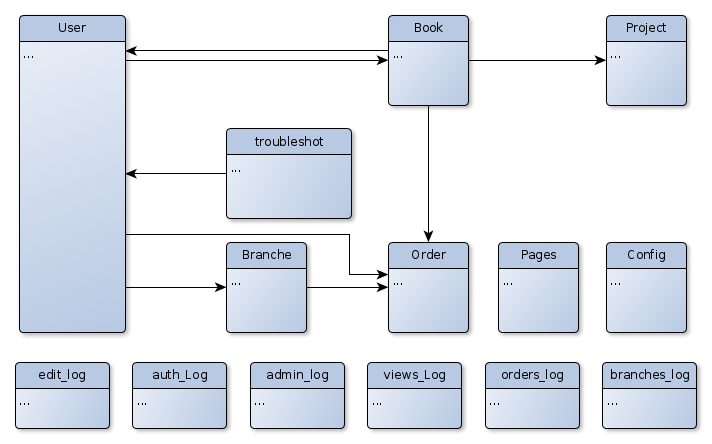
\includegraphics[scale=0.5]{./img/grap_db.png}
\end{array}$
\end{center}
\caption[Diagram databáze]{Diagram kolekcí v databázi aplikace.}
\end{figure}

\subsubsection{Users}
Kolekce uživatelů je nedílnou součástí každého informačního systému, slouží k přihlašování uživatelů i ke správě zaměstnanců a určování práv v aplikaci.
\begin{codeframe}
  \begin{verbatim}
email:
  type: String
  required: true
  unique: true
  index: true
img:
  type: Schema.Types.Mixed
locale:
  type: String
name:
  type:String
  required:true
surname:
  type:String
  required:true
tokenMaxAge:
  type: Number
  required: true
  default: config.options.maxAge
cookieTokenSalt:
  type: String
  required: true
storageTokenSalt:
  type: String
  required: true
passwordSalt:
  type: String
  required: true
password:
  type: String
  required: true
address:
  [
    state: String
    city: String
    street: String
    postal: Number
    home_number: Number
    type: String
  ]
billing_address:[
  state: String
  city: String
  street: String
  postal: Number
  home_number: Number
  type: String
]
tel:
  type:String
posititon:
  type:String
  required:false
    \end{verbatim}
\end{codeframe}
První část dokumentu uživatele se zabívá klasickými uživatelskými informacemi. K čemu slouží všechny salty bude probráno v sekci přihlášování uživatelů.

\begin{codeframe}
  \begin{verbatim}
orders:
  [
    type: Schema.Types.ObjectId
    ref: "Order"
  ]
projects:
  [
    type: Schema.Types.ObjectId
    ref: "Project"
  ]
whished_books:
  [
    type: Schema.Types.ObjectId
    ref: "Book"
  ]
payed_e_books:
  [
    type: Schema.Types.ObjectId
    ref: "Book"
  ]
payed_books:
  [
    type: Schema.Types.ObjectId
    ref: "Book"
  ]
favourite_books:
  [
    type: Schema.Types.ObjectId
    ref: "Book"
  ]
    \end{verbatim}
\end{codeframe}
Další část dokumentu se zabívá především referencemi na knihy. Uživatel může mít velké množství objednávek, které samostatně obsahují všechny uživatelovi informace. Každý uživatel může tvořit také knihy takže mu náleží kolekce projektů, může si přát knihy, které mu mohou kupovat známí a~může mít označeny své oblíbené knihy. Velmi důležitou položkou jsou pak zaplacené knihy, podle tehoto pole systém pozná, které knihy může uživatel stáhnou ve formátu PDF nebo jestli si je koupil v~tiskovém vydání.

\begin{codeframe}
  \begin{verbatim}
roles:
  type: [String]
  default: ['anonymous']
special:
  canRead:
    [
      collection: String
      reference: String
    ]
  canEdit:
    [
      collection: String
      reference: String
    ]
    \end{verbatim}
\end{codeframe}
Následu část zabívající se právy uživatele, uživatel může mít definované role a~zvláštní práva pro čtení a~zápis pro různé kolekce.

\begin{codeframe}
  \begin{verbatim}
User-Agent:String
remoteAddress:String
X-Forwarded-For:String
last_login:
  type:Date
  default: Date.now
  \end{verbatim}
\end{codeframe}
Důležité je také uchovávat informace o~posledním přihlášení uživatele a~odkuk byl uživatel přihlášen. Především kvůli bezpečnosti uživatele, kdy uživatel nebo i~systém automaticky může některé přihlášení vyhodnotit jako falešné, především na základě geolokačních dat IP adresy. Více údajů o~předchozích přihlášeních, lze pak vyčíst z~Auth logu \odkazNaKapitolu{database:log}.

\begin{codeframe}
  \begin{verbatim}
meta: [
  key: String
  value: String
]
updated_at:
  type:Date
  default: Date.now
created_at:
  type:Date
  default: Date.now
  \end{verbatim}
\end{codeframe}
Poslední částí, se bude opakovat téměř ve všech kolekcích takže nebude dále uvedena. Zabívá se především dalších popisků objektu a~časy vytvoření a poslední úpravy.

\subsubsection{Books}
Tou nejdůležitější částí databáze knihkupectví jsou knihy, pro ty je určena kolekce \it{book}, která zajišťuje kompletní informace o~knize od jejího popisu až po informace o~historii ceny prodejích a autorovi.
\begin{codeframe}
  \begin{verbatim}
name:
  type: String
  required: true
  index: true
author:
  name:
    type: String
    required: true
  description: String
  img:
    data: Buffer
    contentType: String
url:
  type: String
owner:
  type: Schema.Types.ObjectId
  ref: "User"
img:
  small:
    data: Buffer
    contentType: String
  big:
    data: Buffer
    contentType: String
genres:[
  name: 
    type: String
    index: true
]
keywords:
  type:String
  required:false
pages:
  type: Number
  required: true
  \end{verbatim}
\end{codeframe}
První část dokumentu se zabívá popisem knihy a~jejím autorem. Přesto, že~by se po zvyklostech z~SQL databází mohlo zdát výhodnější mít autory v~samostatné kolekci není tomu tak, v~tomto případě se stáhnou informace o~autorovi společně s~knihou a~informace o~autorovi se mohou u~každé knihy měnit např. podle období kdy knihu napsal. Dotaz na vyhledání autora v kolekci podle jména není nijak složitý. Následující vrátí všechny knihy, které~mají ve jméně autora řetězec \it{George}.
\begin{codeframe}
  \begin{verbatim}
name = 'George'
book.find(
  author.name: new RegExp('^'+name+'$', "i"), (err, doc)->
    console.log doc
)
  \end{verbatim}
\end{codeframe}
U náročnějšího systému by bylo pak zřejmně vhodné vytvořit pro autory ještě samostatnou kolekci, ale~údaje o~autorovi zanechávat také v~knihách a~kolekci autorů používat pouze pro vyhledání knih konkrétních autorů.

\begin{codeframe}
  \begin{verbatim}
commets:[
  {
    author:
      type: String
      require: true
    coment:
      type: String
      require: true
    user:
      type: Schema.Types.ObjectId
      ref: "User"
  }
]
rating:[
  {
    value:
      type: Number
      require: true
    user:
      type: Schema.Types.ObjectId
      ref: "User"
  }
]
review:[
  {
    title:
      type: String
      require: true
    user:
      type: Schema.Types.ObjectId
      ref: "User"
    content: String
  }
]
  \end{verbatim}
\end{codeframe}
Další v~kolekci jsou pak data, kterými přispívají uživatelé. Jsou možné přidávat komentáře, hodnotit knihy a~psát recenze.

\begin{codeframe}
  \begin{verbatim}
buyers:[
  type: Schema.Types.ObjectId
  ref: "User"
]
number_of_sales:
  type:Number
  required:false
avaible:Boolean
delivery_msg:String
price:
  type:Number
released:Date
public_from:Date
buy_allowed_from:Date
description:String
publisher:String
price_hystory:[
  {
    date:
      type:Date
      default: Date.now
    value:
      type:Number
  }
]
  \end{verbatim}
\end{codeframe}
Poslední část dokumentu je pouze statistická, je zde výčet uživatelů, kteří si knihu koupily, historie ceny, dostupnost knihy a~informace o~vydání.

\subsubsection{Orders}
Objednávka je v SQL databázích většinou předmětem velkého množství relací na uživatele adresy, schvalování, dopravu apd,… Toto všecho NoSQL databáze řeší velmi elegantně v jediném dokumentu. Bez jakých kolik relací, které vy vyžadovali další odkazování. Navíc pokud je obejdnávka již jendou vytvořena neměl by její obsah být pozměněn referncemi.
\begin{codeframe}
  \begin{verbatim}
  user:
    name:
      type:String
      required: true
    surname:
      type:String
      required: true
    tel:
      type:String
      required: true
    email:
      type:String
      required: true
    user:
      type: Schema.Types.ObjectId
      ref: "User"
  price:
    type:Number
    required: true
  \end{verbatim}
\end{codeframe}
První část obsahuje informace o~kupujícím včetně reference na něj, ale v případě, že v budoucnu dojde ke smazání kupujícího, data o~obchodu sním jsou stále zaznamenána a~konzistentní.

\begin{codeframe}
  \begin{verbatim}
  items:[
    name:
      type: String
      required: true
      index: true
    author:
      type: String
      required: true
    price:
      type:Number
      required: true
    released:Date
    description:String
    pages:
      type: Number
    book:
      type: Schema.Types.ObjectId
      ref: "User"
  ]
  \end{verbatim}
\end{codeframe}
Velmi důležitý je seznam zakoupených položek. Opět je část základních data zkopírována do dokementu aby nedošlo ke~změnám v~objenávkách následkem změny reference.

\begin{codeframe}
  \begin{verbatim}
  confirmed:Boolean
  states:[
    title:String
    description:String
    date:Date
      default: Date.now
    user:
      type: Schema.Types.ObjectId
      ref: "User"
  ]
    \end{verbatim}
\end{codeframe}
Objednávka má samozřejmně svou historii a~to od chvíle jejího vytvoření až do chvíle jejího zrušení. Proto jsou v~této části definovány změny v~objednávce. Pokaždé když objednávka postoupí schvalovacím procesem, nebo změnou zapíše se zpráva co se stalo a~kdo akci vyvolal.

\begin{codeframe}
  \begin{verbatim}
  custom_id:String
  custom_description:String
  payed:Boolean
  billing_address:
    state: String
    city: String
    street: String
    postal: Number
    home_number: Number
    type: String
  destination_address:
    state: String
    city: String
    street: String
    postal: Number
    home_number: Number
    type: String
  pay_method:
    name:
      type:String
      required: true
    card_number:
      type:Number
  delivery_method:
    name:
      type:String
      required: true
    price:
      type:Number
      required: true
    branche:
      name: String
      city: String
      street: String
      postal: Number
      home_number: Number
      tel: Number
      \end{verbatim}
\end{codeframe}
Poslední část se zabívá obchodem samotným. Uživatel má možnost zvolit vlastní identifikator objednávky, metodu platby, kam bude objednávka zaslána, kam fakturována a~jestli byla objednávka z~e-shopu nebo z~pobočky.//

\subsubsection{Project}

\subsubsection{Branches}
Knihkupetví většinou nemají pouze internetový obchod, ale také kammené pobočky. Pro držení informací o~pobočkách slouží kolekce Branches.
\begin{codeframe}
  \begin{verbatim}
  name:
    type: String
    required: true
  address:
    state: String
    city: String
    street: String
    postal: Number
    home_number: Number
    type: String
  contacts:[
    {
      name: String
      description: String
      tel: String
      fax: String
      email: String
    }
  ]
  employes:[
    {
      name:String
      position:String
      paychecks:[
        priod_from:Date
        priod_to:Date
        sended:Date
        sum:Number
        info:[
          title:String
          score:string
        ]
      ]
      user:
        type: Schema.Types.ObjectId
        ref: "User"
    }
  ]
  \end{verbatim}
\end{codeframe}
Kolekce poboček musí samozřejmně obsahovat informace o~pobočce samotné a také o jejích zaměstatnancích zaměstnacích, platech zaměstnanců apd,…

\begin{codeframe}
  \begin{verbatim}
  books_on_sale:[
    {
      type: Schema.Types.ObjectId
      ref: "Book"
    }
  ]
  books_to_arrive:[
    {
      order_date: Date
      arrival_date: Date
      state:String
      book:
        type: Schema.Types.ObjectId
        ref: "Book"
    }
  ]
  orders:[
    {
      type: Schema.Types.ObjectId
      ref: "Order"
    }
  ]
    \end{verbatim}
\end{codeframe}
Každá pobočka si navíc musí vést informace o~knihách dostupných na pobočce, knihách které má objednány a~uskutečněných prodejích.

\subsubsection{Config}
config je pouze jednoduchá key:value databáze určená ke změnám v~prostředí aplikace, tyto změny pak nepotřebují restart nodejs serveru. Vhodným řešením takovéto kolekce, je pak cachování do jiné NoSQL databáze jako je Redis nebo Memcache.\\

\begin{codeframe}
  \begin{verbatim}
config.groups:[
  name:String
  colection_r:[String]
  colection_w:[String]
  actions_allowed:[String]
  routes_allowed:[String]
]
    \end{verbatim}
\end{codeframe}
Klíč \it{groups} zajištuje nastavení skupin a~přístup k~jednotlivým akcím

\begin{codeframe}
  \begin{verbatim}
config.actions:[String]
    \end{verbatim}
\end{codeframe}
Seznam akcí backendu.

\subsubsection{Troubleshoot}
V případě, že~má uživatel portálu dotaz, je k~dispozici troubleshoot kolekce, která zajišťuje komunikaci uživatelů s~provozovatelem služby.\\

\begin{codeframe}
  \begin{verbatim}
title:
  type: String
  required: true
msg:
  type: String
user_started:
  name:String
  user:
    type: Schema.Types.ObjectId
    ref: "User"
user_involved:[
  name:String
  user:
    type: Schema.Types.ObjectId
    ref: "User"
]
alert_users:[
  type: Schema.Types.ObjectId
  ref: "User"
]
stage:
  type: String
priority:
  type: String
conversation:[
  msg:
    type: String
  stage_change:Boolean
  priority_change:Boolean
  user:
    name:String
    user:
      type: Schema.Types.ObjectId
      ref: "User"
]
    \end{verbatim}
\end{codeframe}
Každé vlákno problémů má svůj titulek úvodní zprávu, jménu uživatele, který~ho vytvořil, seznam uživatelů zapojených do řešení, seznam uživatelů, kteří jsou informováni o~změnách ve vlákně. Každé vlákno má navíc prioritu a~fázi ve, které se nachází. Samozřejmě je možné přidávat zprávy, které mohou být navíc označeny jako změna priority nebo změna stavu.


\subsubsection{Pages}
Kolekce statických stránek. Jedná se o~kolekci editovatelných webových stránek. Např. informace o~obchodu, kontakty apd,…

\begin{codeframe}
  \begin{verbatim}
  title:
    type: String
    required: true
  url:
    type: String
    index: true
  content:String
  img:[
      name:String
      img:
        data: Buffer
        contentType: String
  ]
  meta: [
      {
        key: String
        value: String
      }
    ]
  \end{verbatim}
\end{codeframe}
Kolekce odpovídá struktuře bězné webové stránky. Obsahuje odkaz na stránku titulek, obsah, obrázky a~meta tagy velmi důležité především pro SEO optimalizace.

\subsubsection{Logs}
Důležitým aspektem u~každého webového systému jsou logy a~logování co největšího množství událostí, nejenom pro statistické údaje, ale i~pro případ stížností ze~strany klienta ať už kvůli ztrátě dat nebo nefunkčnosti funkcí.

Pro logování má informační systém několik logů, každý určený pro jiný typ události.

\begin{description}\label{database:log}
\item[Edit log] slouží pro zaznamenávání událostí spojených s~úpravou a~vytváření knih.
\item[Auth log] log pro zaznamenávání událostí souvisejících s~přihlašováním. Např. uživatel se přihlásil, odhlásil, registroval, zadal špatné heslo, přišel do aplikace apd,…
\item[Admin log] v tomto logu se zaznamenávají události spojené s~administrací. Pokud uživatel s~vyšším oprávněním něco změní, zobrazí se tato událost zde.
\item[Views log] tento log slouží především pro statistiky zaznamenávají se zde informace o~tom, který uživatel kdy navštívil kterou stránku.
\item[Orders log] v tomto logu se zaznamnávají události související s~objednáváním knih jako, uživatel vytvořil objednávku, přidal položku, zaplatil objednávku, zrušil objednávku apd,…
\item[Branches log] záznam událostí spojených s~pobočkami.
\end{description}
logovací kolekce vypadají velmi podobně, proto bude popsána obecná struktura záznamu.

\begin{codeframe}
  \begin{verbatim}
_user_id
  \end{verbatim}
\end{codeframe}
reference na uživatele, který vyvolal akci, pokud není uvedena je uživatel anonymní.

\begin{codeframe}
  \begin{verbatim}
_page_id
  \end{verbatim}
\end{codeframe}
reference na stránku. (používá se u view logu aby bylo možné získat statistiku navštívené stránky a~auth logu aby bylo možné zjisti na, kterou stránku se uživatel pokusil přihlásit)

\begin{codeframe}
  \begin{verbatim}
url
  \end{verbatim}
\end{codeframe}
URL adresa kde byla událost vyvolána

\begin{codeframe}
  \begin{verbatim}
message
  \end{verbatim}
\end{codeframe}
popis události

\begin{codeframe}
  \begin{verbatim}
event
  \end{verbatim}
\end{codeframe}
název události

\begin{codeframe}
  \begin{verbatim}
type
  \end{verbatim}
\end{codeframe}
typ události (ERROR, INFO, DEBUG, WARN)

\begin{codeframe}
  \begin{verbatim}
User-Agent
  \end{verbatim}
\end{codeframe}
pro lepší vyhodnocení události a~případný troubleshoot jsou zaznamenány informace o~prohlížeči

\begin{codeframe}
  \begin{verbatim}
remoteAddress
  \end{verbatim}
\end{codeframe}
záznam IP adresy, ze která záznam vyvolala

\begin{codeframe}
  \begin{verbatim}
X-Forwarded-For
  \end{verbatim}
\end{codeframe}
stejný záznam jako předchozí sloužící pro získání IP adresy v~případě,že se aplikace nachází za proxy serverem.

\subsection{Budoucí vývoj}
MongoDB a~jeho absence schémat zajišťuje snadnější rozšiřitelnost aplikace, není třeba nijak zvláště řešit relace mezi kolekcemi a~už vůbec ne schéma, protože MongoDB nemá žádné schéma. Prakticky stačí změnit schéma v~mongoose, které je pouze aplikační a~MongoDB o~něm neví, a restartovat aplikace (nebo provést deploy).\\

Z funkcionálního hlediska pak budoucí vývoj záleží na požadvavcích zákazníka, prakticky by pak další vývoj pravděpodobně zahrnoval rozšíření dat, které jsou zaznamenávány o~uživateli aby mu pak aplikace sama nabízela knihy a~informavala o~novinkách, které uživatel může pravděpodobně chtít, na základě procházených, koupených knih nebo i~informací o~procházení jiných webových stránek.\\

Dalším bodem rozšíření je pak reklama, jak už reklama na položky portálu samotného tak i~placená inzerce dalších portálů a~služeb.\\

\subsection{Zabezpečení}
MongoDB má vlastní systém zabezpečení, který spočívá v~několika systémových rolích vlastním ACL a~omezení přístupu uživatelů k~databázím a~kolekcím. Ovšem aplikace reálně potřebuje přístup jak ke čtení tak k~zápisu do své databáze takže není na místě řešit jakékoliv složitější práva. Ta by mohla přijít vhod v~případě rozdělení aplikace na několik samostatných rozhraní, které by nepotřebovali např. přístup do některých kolekcí nebo zápis do nich. Takový případ by však nastal v~případě obrovských návštěvností a~jak už bylo řečeno penetrace rozhraní a~zařízení přistupujích do databáze.\\

Dalším faktorem zabezpečení je pak zabezpečení serverové. V případě zabezpečení databází obecně, je na snadě zamezit maximálně přímé interakce uživatele a~databáze. Pokud není databáze sdílená a~nepotřebují přístup další externí uživatelé, což je případ spíše multihostingů, kde je většinou otevřený port přímo do databáze nebo je nabízeno rozhraní pro databázi (PHPMyAdmin pro MYSQl, pro MongoDB např. RockMongo). Proto je většinou přístupový bod do databáze možný pouze z~místní sítě aplikace tj. z~jejího aplikačního clusteru. V~tomto nanejvíš vhodném případě je pak přítup do databáze buď přímý přes databázový port nebo přes nějaké rozhraní pro databázi (RockMongo).V~takovém případě je pak třeba vytvořit v~místní síti aplikace server pro vzdálený přístup, vhodným řešením je např. OpenVPN nebo jiný SW pro vzdálený přístup nebo připojení počítače do vzdálené místní sítě v~Internetu.

\subsubsection{Nastavení zabezpečení MongoDB}
Zabezpečení MongoDB databáze je velmi jednoduché a~lze jej sprovoznit pomocí MongoDB cli. Nejprve je třeba spustit program \it{"mongo"}, který je standardní součástí

\section{\upc{Backend}}\label{sec:backend}
O část aplikace na straně serveru se stará NodeJS server postavený frameworku express spolu ODM mongoose pro práci s~databází. 

\subsection{Struktura}
\begin{figure}[h]
\begin{center}$
\begin{array}{c}
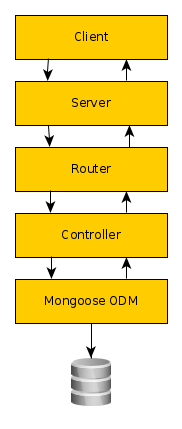
\includegraphics[scale=0.5]{./img/grap_backend.png}
\end{array}$
\end{center}
\caption[Diagram API]{Diagram prostupu struktury backendu aplikace.}
\end{figure}

\subsection{API}
\subsubsection{/api/v1/me}
\subsubsection{/api/v1/book}
\subsubsection{/api/v1/user}
\subsubsection{/api/v1/branch}
\subsubsection{/api/v1/order}
\subsubsection{/api/v1/project}
\subsubsection{/api/v1/page}
\subsubsection{/api/v1/log}

\subsection{Zabezpečení}
\subsection{Přihlášení a soukromí uživatelů}
\subsection{Ochrany proti útoků}
\subsubsection{JSONP}
\subsubsection{XSS}
\subsubsection{CSRF}

\section{\upc{Frontend}}\label{sec:frontend}
\subsection{Komponenty}
\subsubsection{Store (e-shop)}\label{sec:store}
\subsubsection{Create (správa vlastních knih)}\label{sec:create}
\subsubsection{Edit (editor knih)}\label{sec:edit}
\subsubsection{Finance}\label{sec:finance}
\subsubsection{Storage (pobočky a sklady)}\label{sec:storage}
\subsubsection{Statistics (statistiky)}\label{sec:stats}
\subsubsection{Admin (administrace)}\label{sec:admin}


\section{\upc{Gulp}}
Gulp je používán pro sestavení frontendu aplikace, možné je sestavit aplikaci pro produkční a~vývojové účely. Gulp má pro to dva základní tasky \it{dev} a~\it{prod}. Gulp konkrétně sestavuje javascript pomocí browserify, vytváří sprity\footnote{sprite se požívá u~webu pro snížení počtu requestů při načítání. Spojuje obrázky do jednoho velkého obrázku, ze kterého jsou obrázky v~CSS referoncovány pomocí souřadnic a~velikosti }, optimalizuje obrázky, překládá LESS styly na CSS, převádí html soubory do angularové templateCache, takže se všechny views stáhnou spolu s~aplikací, a~obnovuje prohlížeč při změnách v~projektu.
\subsection{Struktura}
Gulp čte v~adresáři kde je spuštěn soubor \it{Gulpfile.js}, ten v~tomto projektu pouze načítá soubor \it{gulp/index.js}. Načtou se všechny soubory ve složce \it{gulp/tasks} a~následně spustí task určený paramentrem příkazu \it{gulp}.

\subsection{Development/Production}
Development prostředí oproti produkčnímu nastavuje některé podrobnější výpisy a~především neprovádí optimalizaci kódu a~obrázků.\\

\begin{description}
\item[Tasky:]

\item[Browserify] - Jak už bylo řečeno Browserify překládá zdrojové kódy v~coffeescriptu na javascript. Navíc má aplikace několik prostředí, kde má každé vlastní kód. Proto je vytváření prostředí ve smyčce.
\begin{codeframe}
  \begin{verbatim}
var enviroments = ["editor","store","admin"]
enviroments.forEach(function (element, index, array) {
  return browserify({
      entries: ['./src/app/'+element+'.coffee'],
      extensions: ['.coffee'],
      transform: ["coffeeify","brfs","envify","browserify-shim"]
  })
  .bundle({debug: true})
  .on('error', handleErrors)
  .pipe(source(''+element+'.js'))
  .pipe(gulp.dest('./assets/js/'))
  .pipe(livereload());
})
    \end{verbatim}
\end{codeframe}

\item[Clean] - Clean pouze čistí projekt před buildem aby ve složce kam bude buildováno nezůstaly staré soubory.
\begin{codeframe}
  \begin{verbatim}
gulp.task('clean', function() {
return gulp.src(["./build", "./tmp/**/*"], {
      read: false
    }).pipe(clean());
});
  \end{verbatim}
\end{codeframe}

\item[Images] - Images především kopíruje obrázky se zdrojové složky, v~produkčním prostředí pak obrázky ještě optimalizuje. \it{pozn. cesta k souboru *.\_NS.png je přítomna, protože všechny png soubory jsou automaticky převáděny do spritu, kromě souborů se~sufixem "\_NS", které jsou zpracovány právě zde.}
\begin{codeframe}
  \begin{verbatim}
gulp.task('images', function() {
return gulp.src('./src/images/**/*{.ico,.svg,.gif,_NS.png}')
  .pipe(changed(dest))
  .pipe(imagemin())
  .pipe(gulp.dest('./build/images'));
});
  \end{verbatim}
\end{codeframe}

\item[Less] - Task Less při svém volání vždy spustí task SPRITES. Je provedena kontrola pomocí \it{recess} a~css kód je automaticky prefixován pro prohlížeče nastavené v~konfiguraci. Při produkčním buildu se pak soubor, ještě minifikuje nastavuje je se mu přípona \it{.min} a~modul \it{rev} vygeneruje do názvu souboru náhodný řetězec, který zaručí, že pokud proběhne změna aplikace na severu, klient stáhne html soubor, a~protože je jiný název css souboru než má uloženo prohlížeč v~cache tak prohlížeč stáhne novou verzi. Pokud by se název souboru nezměnil, načetl by prohlížeč soubor z~paměti a~stránka by byla zastaralá a~třeba i~nefunkční.
\begin{codeframe}
  \begin{verbatim}
gulp.task('LESS', ["SPRITES"], function() {
    return gulp.src("./src/less/main.less")
        .pipe(recess())
        .pipe(less())
        .pipe(autoprefixer(confAutoPrefix))
        .pipe(minifycss())
        .pipe(rename({suffix: ".min"}))
        .pipe(rev())
        .pipe(gulp.dest("./assets/css"))
});
  \end{verbatim}
\end{codeframe}

\item[Sprites] - Sprity především snižují počet requestů při načítání aplikace a zjednodušují vkládání obrázků při kódování. Weby mají často množství obrázkových ikon a~obrázků potřebných pro fungování grafiky, které pokud se načítají samostatně, je na každý obrázek třeba jeden request. Sprite tedy sdružuje všechny obrázky v~jenom velkém obrázku, který je pak z~LESS referencován pomocí mixinu. Pokud se tedy například ve složce \it{src/images} nachází soubor \it{ikona.png}, je vložen do spritu a~je možné jej referencovat kdekoliv v~LESS dokumentu, pokud includuje soubor \it{tmp/sprites.less} jednoduše pomocí mixinu a~proměnné: \it{.sprite(@ikona);}
\begin{codeframe}
  \begin{verbatim}
var spriteConf={
  base64: true,
  name: 'sprite.png',
  style: 'sprites.less',
  cssPath: 'images/',
  processor: 'less'
};
gulp.task('SPRITES', function() {
  return gulp.src(["./src/images/**/*.png", "!./src/images/**/*_ns.png"])
  .pipe(plumber())
  .pipe(sprite(spriteConf))
  .pipe(gulpif('*.png', gulp.dest("./assets/images")))
  .pipe(gulpif('*.less', gulp.dest("./src/less")));
});
  \end{verbatim}
\end{codeframe}

\item[Templates] - Tento task se stará o~převod šablon ze zdrojových souborů. Možné je psát šablony jak v~HTML tak v~JADE. Další možností šablon je pak templateCache, kdy se html převede na javascript, spojí se do jednoho souboru a stáhnou aplikací při prvním načtení.
% Stejně jako sprity, převod html šablon do jednoho javascriptu snižuje také značně počet requestů. Pokud je použite templateCache musí, ale~vývojář počítat stím, že veškeré zobrazování a~skrývání obsahu, např. z~důvodu oprávnění, musí být ošetřeno ve frontendu pomocí AngularJS. Nejedná se ale~o~velkou překážku a~v~případě potřeby může být část šablon ponechána v~html a~stáhnuta pomocí xhr requestu.
\begin{codeframe}
  \begin{verbatim}
gulp.src(["./src/**/*.html"])
.pipe(gulp.dest("./assets/partials"));

gulp.src(["./src/**/*.jade"])
.pipe(jade({
    pretty:true,
    debug:false
}))
.pipe(gulp.dest("./assets/partials"));
  \end{verbatim}
\end{codeframe}

\item[Watch] - Watch pouze hlídá změny v~souborech, pokud se změní soubor, který~hlídá nebo přibide nový, který odpovídá jeho nastavení spustí nastavený task.
\begin{codeframe}
  \begin{verbatim}
gulp.watch('src/**/*.coffee', ['browserify_dev']);
gulp.watch(['!src/images/**/*_NS.png',
  'src/images/**/*.png','src/**/*.less'], ['LESS_DEV']);
gulp.watch('src/images/**/*{.ico,.svg,.gif,_NS.png}', ['images_dev']);
gulp.watch(['src/**/*.html','src/**/*.jade'], ['templates']);
  \end{verbatim}
\end{codeframe}
\end{description}

Konečné řešení pro spojovaní souborů za účelem snížení počtu requestů by měl přinést chystaný protokol \b{HTTP 2.0}, který přinese multiplexování requestů a respons, lepší kompresi a~mnoho jiného.\cite{http2}

\section{\upc{Nasazení aplikace (server,cloud)}}
V~dnešní době, kdy jsou moderní cloudové služby, které umožňují s~minimální počáteční investicí spustit projek prakticky jakékoliv velikosti. Je velmi dobré zvážit cloudové nasazení buď samostatné databáze nebo většinou kompletního projektu. Samozřejmě záleží především na finanční situaci provozovatele naší služby, jejím aktuálním stavu a~návštěvnosti.\\

Cloud řeší především velké počáteční náklady na sprovoznění služby. Díky škálovatelnosti cloudových služeb nemusíme nijak zvlášť řešit jak velké množství prostředků bude potřeba. Není třeba kupovat fyzické stroje nebo pronajímat dedikované servery. Není třeba shánět zaměstnance, kteří by se starali o~chod serverů nebo platit za nějaké manage řešení.\\

Cloud dává možnosti také rozdělení služeb a~jejich chod u~několika poskytovatelů ať už kvůli dalšímu šetření nákladů ( např. pokud bude MongoDB hosting levnější u~jiného posktovatele bude u~jednoho aplikační část a~u~druhého databázová část apd,… ) nebo dostupnosti z~globálního hlediska v~různých zemích nebo kontinentech.\\

Díky cloudu můžeme také odhadnout náklady a~nároky koupi vlastní serverové infrastruktury, protože po dobu provozu v~cloudu, by bylo nasbíráno velké množství metrik a~následně odhadnuty nároky na vlastní řešení.\\

Velmi vhodným je pak hybridní řešení, kdy je část aplikace provozována na vlastním serveru a~část v~cloudu. Často je v~cloudu provozována především databázová část. \\

V případě koupi vlastní serverové infrastruktury, je třeba myslet na vysokou dostupnost služby tzv. HA\footnote{HA - High Avaibility - dva nebo více serverů jsou vzájemnými klony, a~v~případě výpadku jednoho, nebo více, serverů výpadek nepocítí koncový uživatel, maximálně může dojít ke zpomalení služby v~případě, že by výkon po výpadku byl nedostatečný.}. Nestačí tedy koupit jeden fyzický stroj a~něm provozovat službu. Je třeba koupit minimálně dva stroje a~pokud jeden vypadne zastoupí jej server druhý. Takové řešení má, ale své nevýhody, ta největší je především to, že druhý server běží a~spotřebovává energii naprosto zbytečně přičemž vyžaduje stejnou údržbu a~hrozí u~něj stejná pravděpodobnost HW chyby jako u~serveru, který je využíván. Proto je vhodné před tyto dva (nebo více serverů) umístít load balancer, který by rovnoměrně rozděloval zátěž mezi ně. Díky load balanceru, jsou servery rovnoměrně využívány a~v~případě výpadku převezmou automaticky všechny požadavky funkční servery.\\

\subsection{MongoDB}
V~rozdělení zátěže a~lepšího škálování služeb přispívá i~samotné MongoDB, které umožňuje sharding několika MongoDB serverů a~replikaci data. Sharding, je ale velmi náročný a~k~sprovoznění shardingu je třeba alespoň 7mi serverů, 3~konfigurační, 2~a~více routerů a~2~a~více replik.\cite{sharding}
\begin{figure}[h]
\begin{center}$
\begin{array}{c}
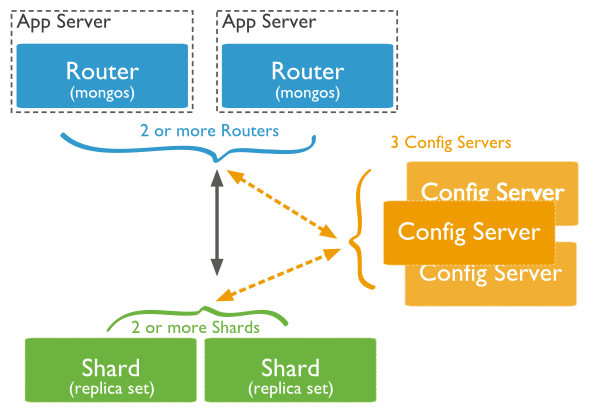
\includegraphics[scale=0.5]{./img/sharding.png}
\end{array}$
\end{center}
\caption[Diagram MongoDB sharding]{Diagram produkčního clusteru pro MongoDB sharding.}
\end{figure}
Sharding je třeba vhodný především pokud množství paměti RAM nedostačuje MongoDB požadavkům, nebo nedostačuje diskový prostor.\cite{sharding}\\

Jednoduší možnosti škálovatelnosti MongoDB je replikace, která je třeba i~v~případě že je použit sharding. Jedná se o~podobný koncept jako je load balancování requestů pro webový server. Je jeden primární MongoDB server, který příjmá požadavky a~přeposílá je pro zpracování sekundárním serverům, které vracejí výsledky.
\begin{figure}[h]
\begin{center}$
\begin{array}{c}
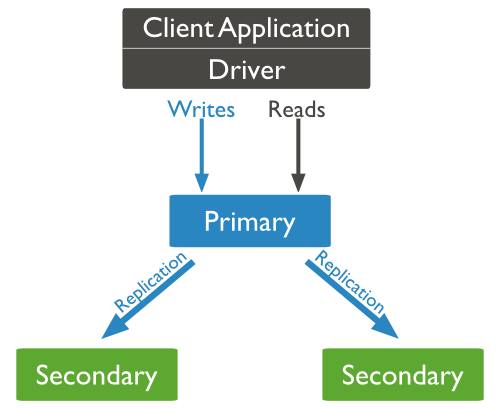
\includegraphics[scale=0.5]{./img/replica.png}
\end{array}$
\end{center}
\caption[Diagram MongoDB replikace]{Diagram jednoduché replikace MongoDB serverů.}
\end{figure}

Škálovatelnost databáze samozřejmně řešíme pouze pokud využíváme vlastní infrastruktury nebo některé cloudové IaaS\footnote{Infrastructure as service - cloudová služba kdy uživatel získá jako by přímo vlastní diskový a~výpočetní výkon a~chová se k~němu jako vlastnímu dedikovanému serveru} služby jako je Amozon EC2. V~případě, že využíváme pro databázi některou ze služeb SaaS\footnote{Service as Service - uživateli je pronajímána pouze služba s~omezeným diskovým prostorem a~výpočétním výkonem} neřešíme škálovatelnost, záleží totiž na tom jaké podpůrné služby si zaplatíme. Takže v~jedné ceně můžeme mít replikovaný cluster včetně záloh.

\subsubsection{Cloudové služby}
Mezi známějsí služby nabízejíci MongoDB patří např. \href{http://mongodirector.com/}{mongodirector.com} nebo \href{http://mongolab.com}{mongolab.com} obě služby jsou podobné, nabízejí MongoDB service v~IaaS službách jiných poskytovatelů např. Amazon AWS, Windows Azure apd,… Infrastruktura je dle zvoleného plánu během několika minut aktivní a~použitelná, bez jakékoliv znalosti nastavení serverů a~řešení jejich zabezpečení. Přičemž ceny vhodné pro provoz poměrně velkých webů začínají kolem 100\$, kdy je možné získat dva replikované mongoDB servery 2GB RAM, 15GB SSD, dvě procesorové jádra a~možnost kdykoliv zvíšit výkon pouhým kliknutím.

\subsection{NodeJS}
V~oblasti nasazení NodeJS aplikací, je opět možnost nasazení buď na vlastní server nebo do cloudu. V~případě vlatního serveru spočívá nasazení v~deploy kódu na server a~spuštění nebo restart nodeJS aplikace.\\

\subsubsection{Vlastní server}
Častou kombinací aplikací zajištějící běh nodeJS aplikace je Proxy server NGINX, Monit pro trvalý běh aplikace, JenkiksCI pro deploy kódu a~například Upstart pro spouštění apliakace samotné.

Nastavení NGINX včetně websockétů a~SSL certifikátu
\begin{codeframe}
  \begin{verbatim}
upstream server {
    server 127.0.0.1:8080;
}
server {
    listen 8085 ssl;
    server_name mojeaplikace.cz;
    ssl_certificate /etc/ssl/mojeaplikace/mojeaplikace.cz.crt;
    ssl_certificate_key /etc/ssl/mojeaplikace/mojeaplikace.cz.key;
    access_log /var/log/nginx/mojeaplikace.log;
    location / {
      proxy_set_header X-Real-IP $remote_addr;
      proxy_set_header X-Forwarded-For $proxy_add_x_forwarded_for;
      proxy_set_header Host $http_host;
      proxy_set_header X-NginX-Proxy true;
      proxy_pass http://server;
      proxy_redirect off;
      proxy_http_version 1.1;
      proxy_set_header Upgrade $http_upgrade;
      proxy_set_header Connection "upgrade";
    }
 }
  \end{verbatim}
\end{codeframe}

Monit se pak stará o~trvalý běh aplikace a~o~její resart po deploy pomocí změny souboru \it{restart}
\begin{codeframe}
  \begin{verbatim}
check process mojeaplikace with pidfile "/var/run/nodejs-mojeaplikace.pid"
    start program = "/sbin/start mojeaplikace"
    stop program  = "/sbin/stop mojeaplikace"
    if failed port 8085
        type tcpSSL protocol http
        request /
        with timeout 10 seconds
        then restart
    depends on mojeaplikace_restart

check file mojeaplikace_restart
    with path /media/data/nodejs/mojeaplikace/restart
    if changed timestamp then restart
  \end{verbatim}
\end{codeframe}

Upstart Script pro spouštění NodeJS aplikací:
\begin{codeframe}
  \begin{verbatim}
#!upstart
description "nodejs mojeaplikace"

start on started mongodb
stop on shutdown
env LOG="/var/log/nodejs/mojeaplikace.log"
env PID="/var/run/nodejs-mojeaplikace.pid"
env nodejsexec="/usr/bin/node"
env app="/media/data/nodejs/mojeaplikace/app.js"
script
    export HOME="/home/nodejs"

    echo $$ > $PID
    exec sudo -u nodejs $nodejsexec $app >> $LOG 2>&1
end script

pre-start script
    # Date format same as (new Date()).toISOString() for consistency
    echo "[`date -u +%Y-%m-%dT%T.%3NZ`] (sys) Starting" >> $LOG
end script

pre-stop script
    rm $PID
    echo "[`date -u +%Y-%m-%dT%T.%3NZ`] (sys) Stopping" >> $LOG
end script
  \end{verbatim}
\end{codeframe}

JenkinsCI pak jenom zkopíruje kód z~GIT repozitáře a~zapíše náhodný řetězec do restart souboru, který zkontroluje monit a~restartuje upstart script.

Ještě je důležité zmínit, že nodejs běží v~jenom vlákně, pokud tedy chceme využít více jader procesoru musíme spustit více instancí a~balancovat mezi nimi, jak už bylo i~zmíněno, nebo~můžeme použít nodeJS cluster, který vytvoří proxyserver a~o~balancování se stará sám.\cite{prezNodeHuge}
\begin{codeframe}
  \begin{verbatim}
cluster = require("cluster")
http = require("http")
numCPUs = require("os").cpus().length
if cluster.isMaster
  i = 0
  while i < numCPUs
    cluster.fork()
    i++
  cluster.on "exit", (worker, code, signal) ->
    console.log "worker " + worker.process.pid + " died"
    return
else
  # HTTP SERVER
  http.createServer((req, res) ->
    res.writeHead 200
    res.end "hello world\n"
    return
  ).listen 8000
  \end{verbatim}
\end{codeframe}
Kód vytvoří nodejs server na portu 8000 a~pro každé jádro procesoru vytvoří jeden worker.\cite{prezNodeHuge}


\subsubsection{Cloud}
V oblasti cloudu je možností také nepočítaně. Mezi nejznámější služby patří např. průkopník v~této oblasti Heroku (\href{http://heroku.com}{http://heroku.com}), NodeJitsu \href{https://www.nodejitsu.com/}{https://www.nodejitsu.com/} nebo relativně nová služba od společnosti Red Hat Openshift \href{https://www.openshift.com/}{https://www.openshift.com/}. Všechny služby jsou velice jednoduché na používání nabízejí jak webové rozhraní pro vytváření aplikací tak jednoduchý deployment pomocí příkazové řádky. Navíc všechny poskytují zároveň MongoDB hosting takže není třeba při startu aplikace využívat externí cloudové služby pro databázi.\\

Vzhledem k~tomu, že je deploy pro všechny cloudové služby prakticky stejný bude uveden příklad pro OpenShift.\\

Pro instalaci a~využití Openshiftu je třeba mít nainstalováno ruby, pak stačí jednoduše nainstalovat gem rhc.
\begin{codeframe}
  \begin{verbatim}
sudo gem install rhc
    \end{verbatim}
\end{codeframe}

Nastavit program rhc, jedná se pouze o~přihlášení a~nastavení SSH klíče.
\begin{codeframe}
  \begin{verbatim}
rhc setup
    \end{verbatim}
\end{codeframe}

Pak stačí vytvořit aplikaci, příkaz nejenom vytvoří aplikační cartridge v~cloudu, ale i~git repozitář v~místě spuštění příkazu.
\begin{codeframe}
  \begin{verbatim}
rhc app create MyApp nodejs-0.10 mongodb-2.6  
  \end{verbatim}
\end{codeframe}

Deploy už je pak pouze vytvoření commitu v~GITu a~deploy pomocí příkazu PUSH.
\begin{codeframe}
  \begin{verbatim}
$cd myapp
$nano app.js
$git commit -a -m "Deploy"
$git push
    \end{verbatim}
\end{codeframe}
webovou adresu aplikace je pak možné získat po přihlášení na webu openshift. Openshift navíc nabízí i~deploy pomocí JenkinsCI nebo Cloud9.


%********************************* Závěr ************************************
\nn{Závěr}

\newpage
%********************************* Seznam Literatury ************************************
\seznamlit{
\bibitem{ngBOOK}Ng-book: The Complete Book on AngularJS [online]. Fullstack io, 2013 [cit. 2014-02-01]. ISBN 978-0991344604. Dostupné z: https://www.ng-book.com/. [e-kniha] 
\bibitem{NodeJS}Mastering Node.js [online]. Packt Publishing, 2013 [cit. 2014-02-01]. ISBN 978-1782166320. Dostupné z: http://visionmedia.github.io/masteringnode/. 
\bibitem{selfPublish}POYNTER, Dan. Dan Poynters self-publishing manual: how to write, print and sell your own book. 15th ed., completely rev. Santa Barbara, Calif.: Para Pub., 2006, 463 p. ISBN 978-156-8601-342.
\bibitem{htmlDesign}DUCKETT, Jon. HTML: design and build websites. Indianapolis, IN: Wiley, c2011, 490 p. ISBN 11-180-0818-9.
\bibitem{TeX}OETIKER, Tobias, Hubert PARTL, Irene HYNA a Elisabeth SCHLEGL. The Not So Short Introduction to LATEX [online]. [cit. 2014-02-01]. Dostupné z: http://www.ctan.org/tex-archive/info/lshort/english/.
\bibitem{nodejsEventArch}http://www.nodejs.cz/co-je-event-driven-architektura/. [e-kniha] 
\bibitem{expressjs}http://expressjs.com/. [e-kniha] 
\bibitem{trendsIS}http://www.businessit.cz/cz/analytici-informacni-systemy-cloud-socialni-crm-business-intelligence.php
\bibitem{abcLinuxuSerialMongo}http://www.abclinuxu.cz/clanky/programovani/lehky-uvod-do-mongodb. [e-kniha] 
\bibitem{angularGITHUB}https://github.com/angular/angular.js. [e-kniha] 
\bibitem{angularJSFolders}http://cliffmeyers.com/blog/2013/4/21/code-organization-angularjs-javascript. [e-kniha] 
\bibitem{angularAnimation} https://docs.angularjs.org/guide/animations [e]
\bibitem{lesscss} http://lesscss.org/ [e]
\bibitem{jade} http://jade-lang.com/
\bibitem{bower} http://bower.io/
\bibitem{hapiJS}http://spumko.github.io/
\bibitem{hapiJSDOC}https://github.com/spumko/hapi/blob/master/docs/Reference.md
\bibitem{mean} http://blog.mongodb.org/post/49262866911/the-mean-stack-mongodb-expressjs-angularjs-and
\bibitem{dart} https://www.dartlang.org/
\bibitem{prezNodeHuge}http://www.slideshare.net/OnModulus/planningforthehorizontal-scalingnode-js-18572644
\bibitem{typeScript} http://www.typescriptlang.org/Tutorial
\bibitem{BASHen}http://www.nodejs.cz/co-je-event-driven-architektura/. [e-kniha]
\bibitem{sharding}http://docs.mongodb.org/manual/core/sharding/.
\bibitem{http2} http://http2.github.io/http2-spec/index.html\#StreamsLayer
\bibitem{MailingListVznikGITu}TORVALDS, Linus.{\it{ LKML.ORG - the Linux Kernel Mailing List Archive}} [online]. 2005-04-07 [cit. 2011-05-26]. Linus Torvalds: Re: Kernel SCM saga. Dostupné z~WWW: \href{http://lkml.org/lkml/2005/4/8/9}{http://lkml.org/lkml/2005/4/8/9}.
\bibitem{GITWEB}CHACON, Scott. {\it{ Git}} [online]. 2005 [cit. 2011-05-26]. Git - Fast Version Control System. Dostupné z~WWW: \href{http://git-scm}{http://git-scm}
\bibitem{GIThelpNastaveni}GitHub Inc.{\it{ Help.GitHub }}[online]. 2011 [cit. 2011-05-26]. Set Up Git (Linux). Dostupné z~WWW: \href{http://help.github.com/linux-set-up-git/}{http://help.github.com/linux-set-up-git/}.
\bibitem{GITmanualMerge}Linux Kernel Organization, Inc. {\it{The Linux Kernel Archives}} [online]. 2006 [cit. 2011-05-26]. Git User’s Manual (for version 1.5.3 or newer). Dostupné z~WWW: \href{http://www.kernel.org/pub/software/scm/git/docs/user-manual.html\#how-to-merge}{http://www.kernel.org/pub/software/scm/git/docs/user-manual.html\#how-to-merge}.
}

%********************************* Seznam zkratek ************************************
\seznamzkr

\begin{tabular}{ll}
LFS & Linux From Scratch \\
\end{tabular}
%********************************* Seznam obrázků ************************************
\seznamobr
%********************************* Seznam tabulek ************************************
%\seznamtab
%********************************* Seznam příloh ************************************
\listofappendices

\priloha{PDF verze bakalářské práce a zdrojový kód v~jazyce LaTeX}

PDF je dostupné na DVD v~portále STAG a~na~internetu\\

\href{https://github.com/zajca/BC.TvorbaLinuxoveDistribuce}{https://github.com/zajca/BC.TvorbaLinuxoveDistribuce}\\


%\section*{PŘÍLOHA P I: ŠABLONA SLOVNĚ.}
\end{document}
